\subsection{Run on GTEx}
Once the model was tuned and adapted to RNA-Sequencing data, it was run on a subset of the GTEx dataset. A subset was chosen randomly in order to reduce the computing time needed. The analysis hereby described took about 2 days to be run on a 16 core CPU, 100GB memory facility. The great amount of memory is needed to temporary store the network configuration at each step of the Monte Carlo simulation.

First of all to rapidly have an information about the interest of the oncoming result the metric above described were considered. In figure~\ref{fig:topic/gtex/oversigma_10tissue/metric_scores} it is represented the V-measure score versus the number of clusters found at different layers.
\begin{figure}[htb!]
    \centering
    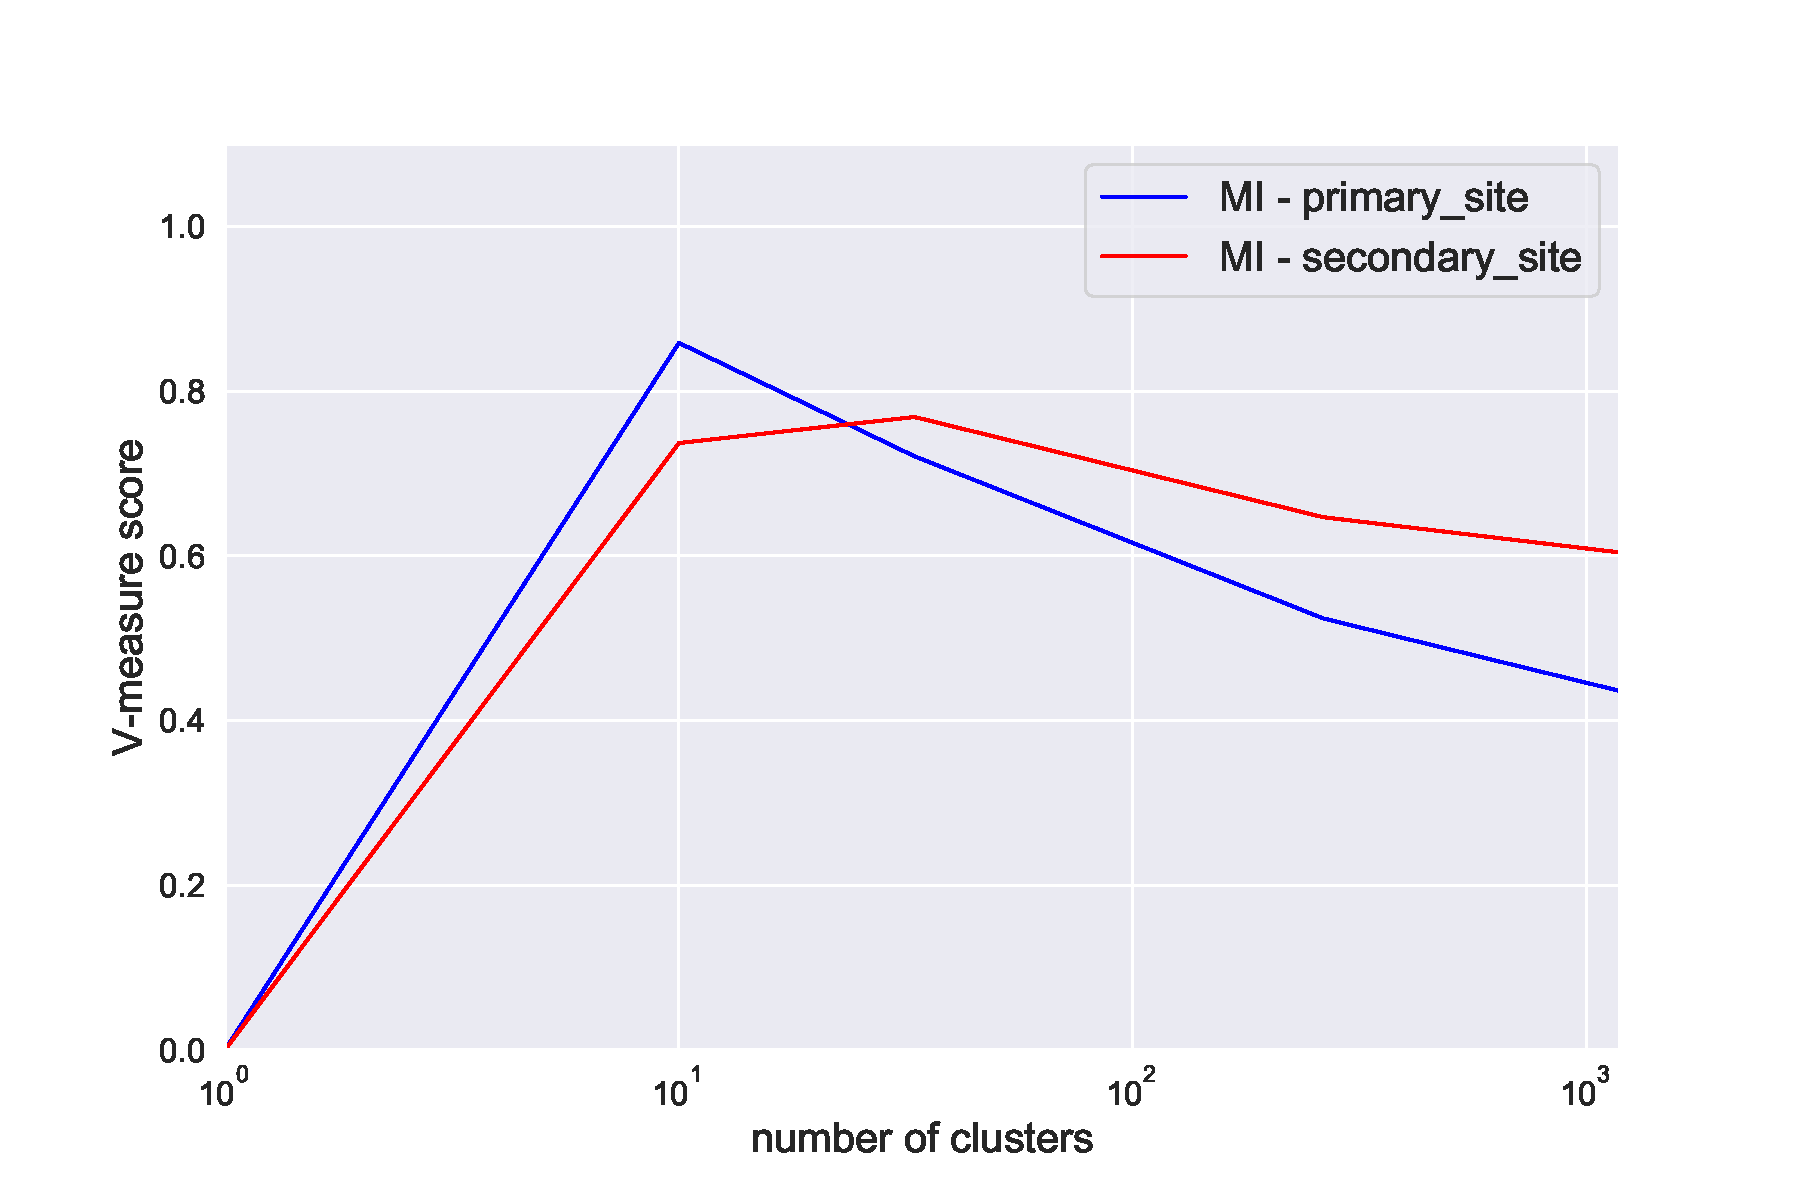
\includegraphics[width=0.9\linewidth]{pictures/topic/gtex/oversigma_10tissue/metric_scores.pdf}
    \caption{Scores across hierarchy. The primary site and secondary site labels are compared.}
    \label{fig:topic/gtex/oversigma_10tissue/metric_scores}
\end{figure}
The result is quite good, the maximum score is over $0.8$. Considering that, for example,~\cite{Farver2018} obtained a similar score considering only homogeneity, this is a quite good result. A second interesting fact is that both the tissue label (primary site) and the sub tissue label (secondary site) obtain such a good score, moreover the the secondary site score's peak is at an higher number of clusters coherently with the fact that there is a greater number of sub tissue labels.
This score can be useful to define at which level of the hierarchy the consequent analysis should be made.

In figure~\ref{fig:topic/gtex/oversigma_10tissue/bipartite_rebuild} the relation between the clusters at different layers it is evident.
\begin{figure}[htb!]
    \centering
    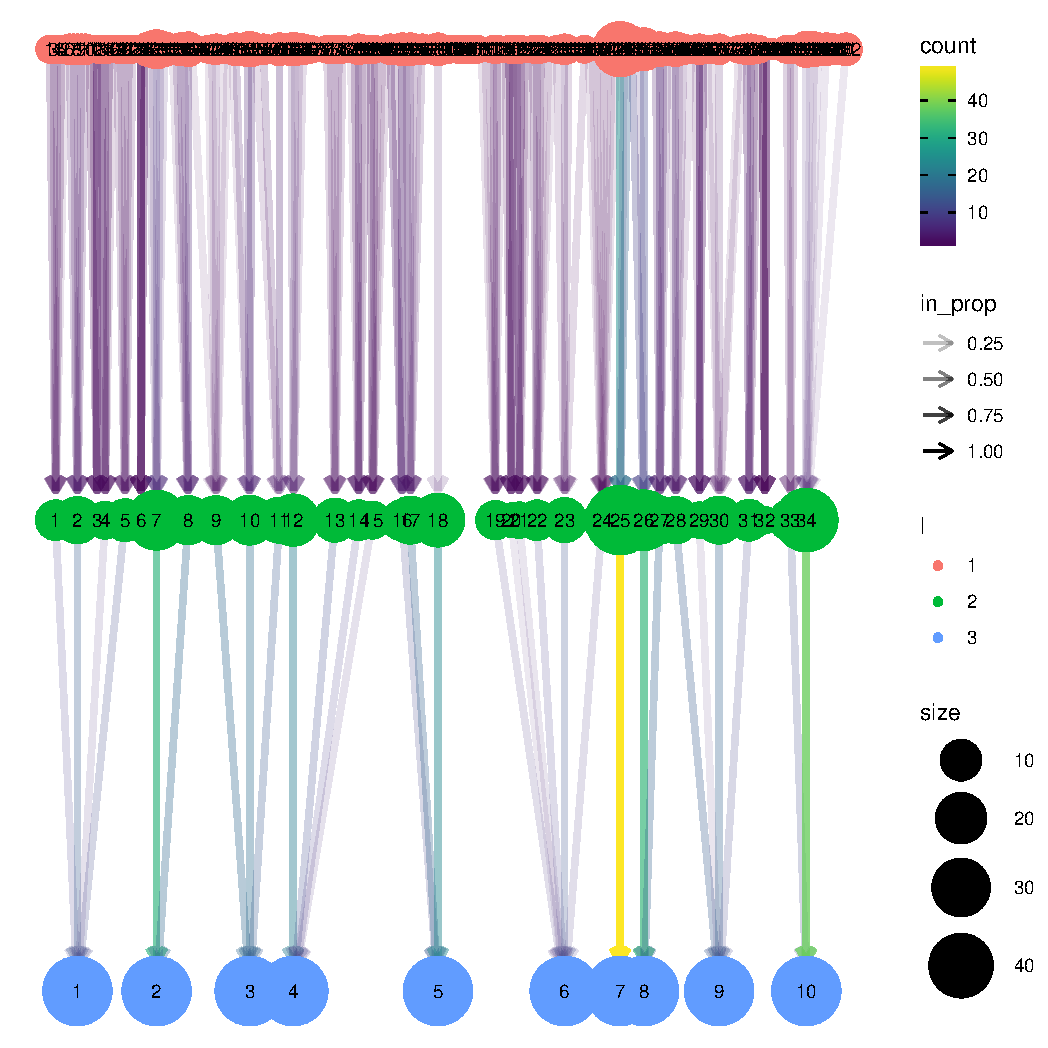
\includegraphics[width=0.8\linewidth]{pictures/topic/gtex/oversigma_10tissue/bipartite_rebuild.pdf}
    \caption{Hierarchy of the files' nodes.}
    \label{fig:topic/gtex/oversigma_10tissue/bipartite_rebuild}
\end{figure}

\clearpage

In figure~\ref{fig:topic/gtex/oversigma_10tissue/clustercomposition_l3_primary_site} each column is a cluster and each color is a tissue of the dataset. It is evident that the majority of the tissue are identified: the first, second, fifth, sixth, eighth and tenth columns are fully and uniformly colored of the same color. These corresponds to an identification of brain, blood, lung, testis and bladder.
\begin{figure}[htb!]
    \centering
    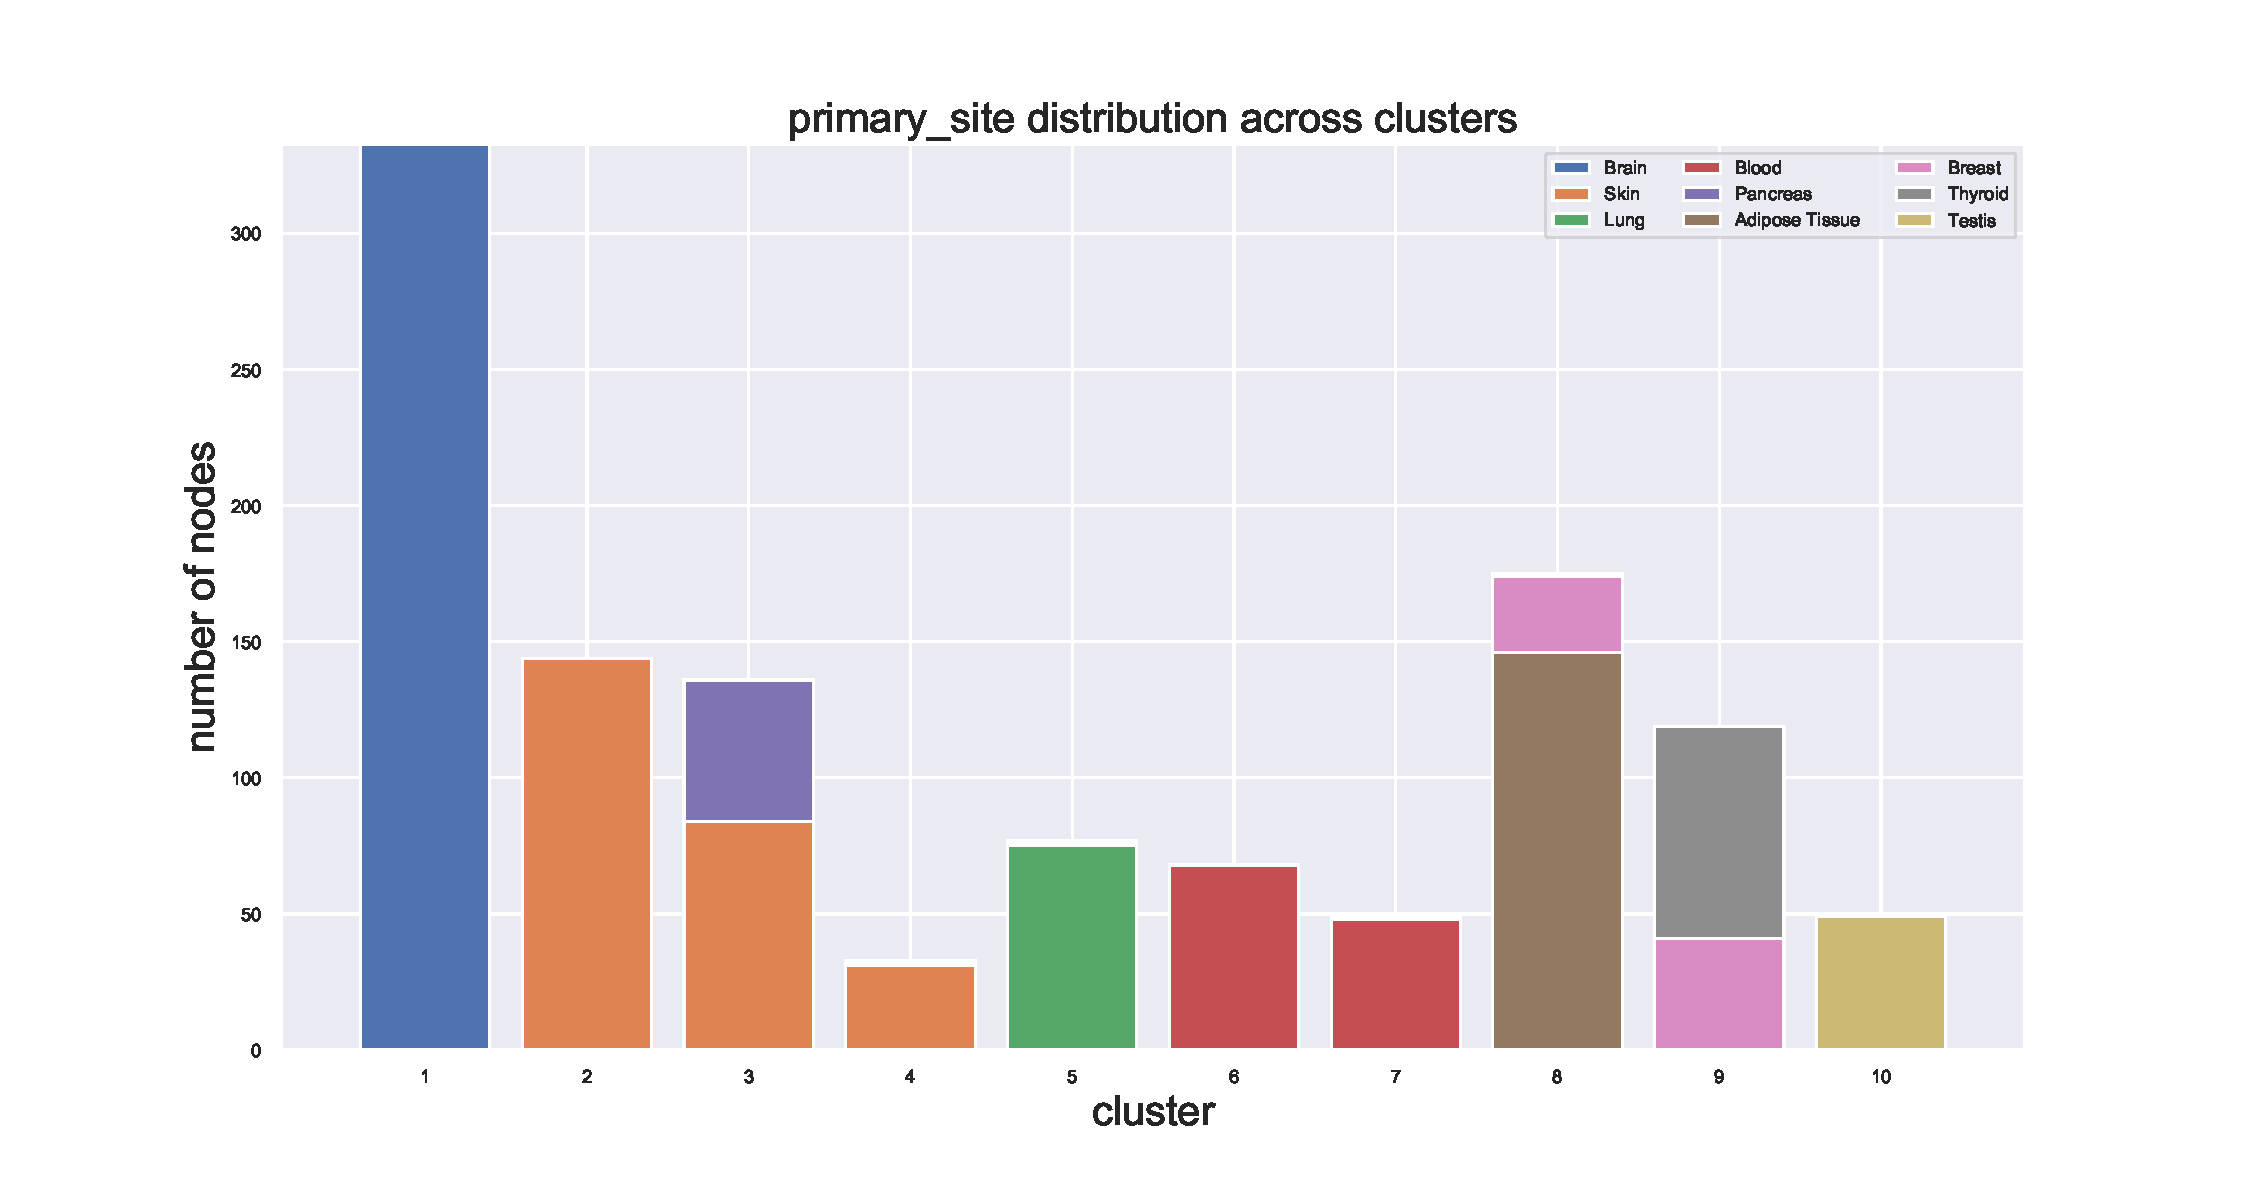
\includegraphics[width=0.9\linewidth]{pictures/topic/gtex/oversigma_10tissue/clustercomposition_l3_primary_site.pdf}
    \caption{Clusters composition at level of the hierarchy with higher score. Each column is a cluster, each color is a label.}
    \label{fig:topic/gtex/oversigma_10tissue/clustercomposition_l3_primary_site}
\end{figure}
A normalised representation of the same clusters the result is still quite interesting and the homogeneity of the clusters is more evident.
\begin{figure}[htb!]
    \centering
    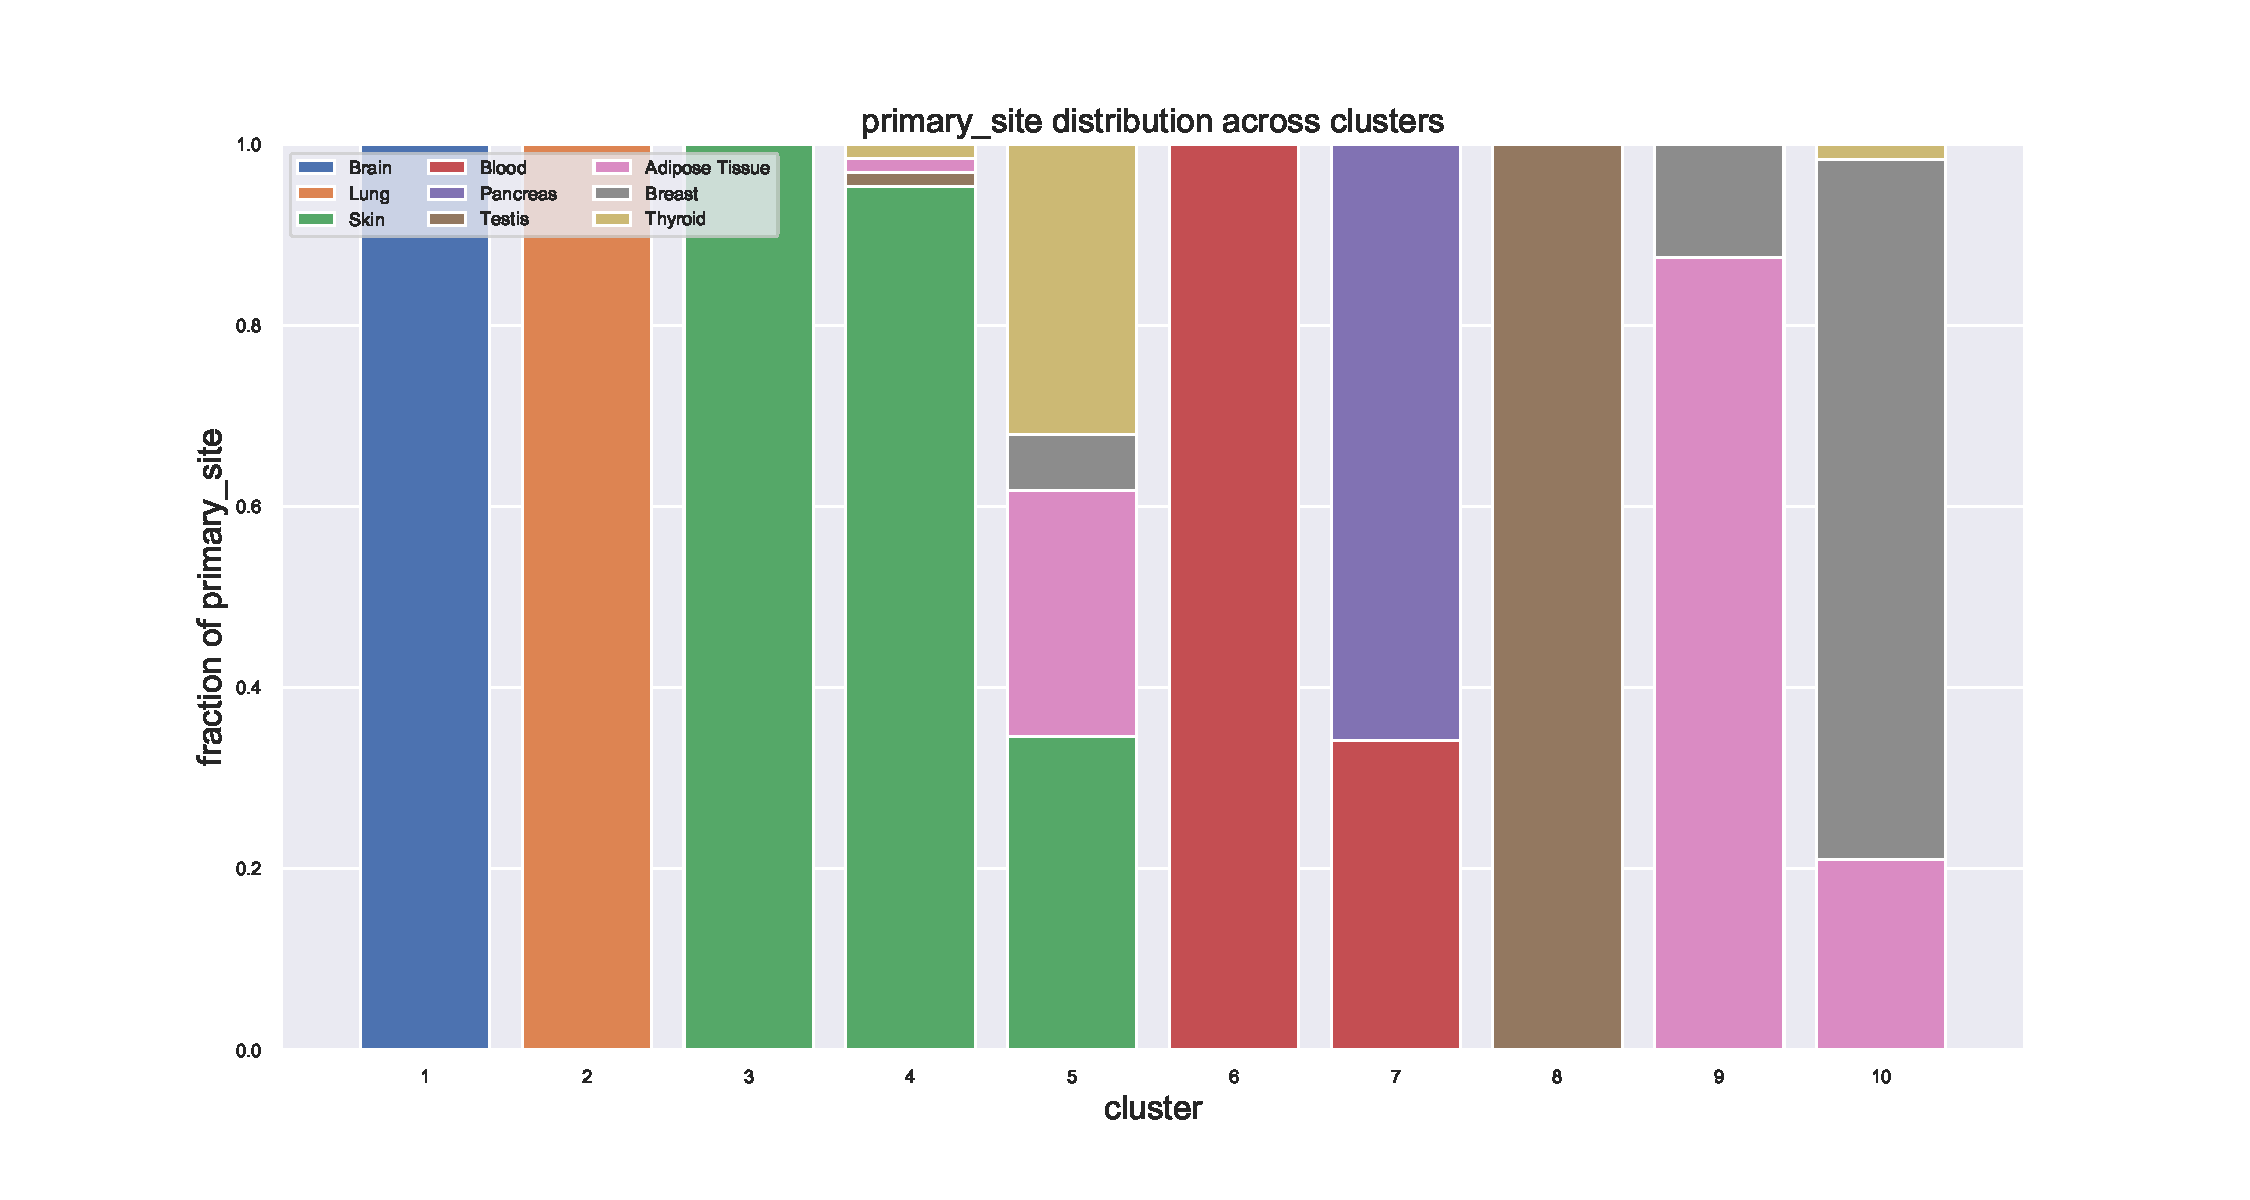
\includegraphics[width=0.9\linewidth]{pictures/topic/gtex/oversigma_10tissue/fraction_clustercomposition_l3_primary_site.pdf}
    \caption{Normalised composition of clusters.}
    \label{fig:topic/gtex/oversigma_10tissue/fraction_clustercomposition_l3_primary_site}
\end{figure}
Going deeper in the hierarchy and looking at a layer with more cluster the result, shown in figure~\ref{fig:topic/gtex/oversigma_10tissue/fraction_clustercomposition_l2_primary_site}, demonstrates that at this point all the the tissues are separated and each cluster is fully of nodes sharing the same tissue.
\begin{figure}[htb!]
    \centering
    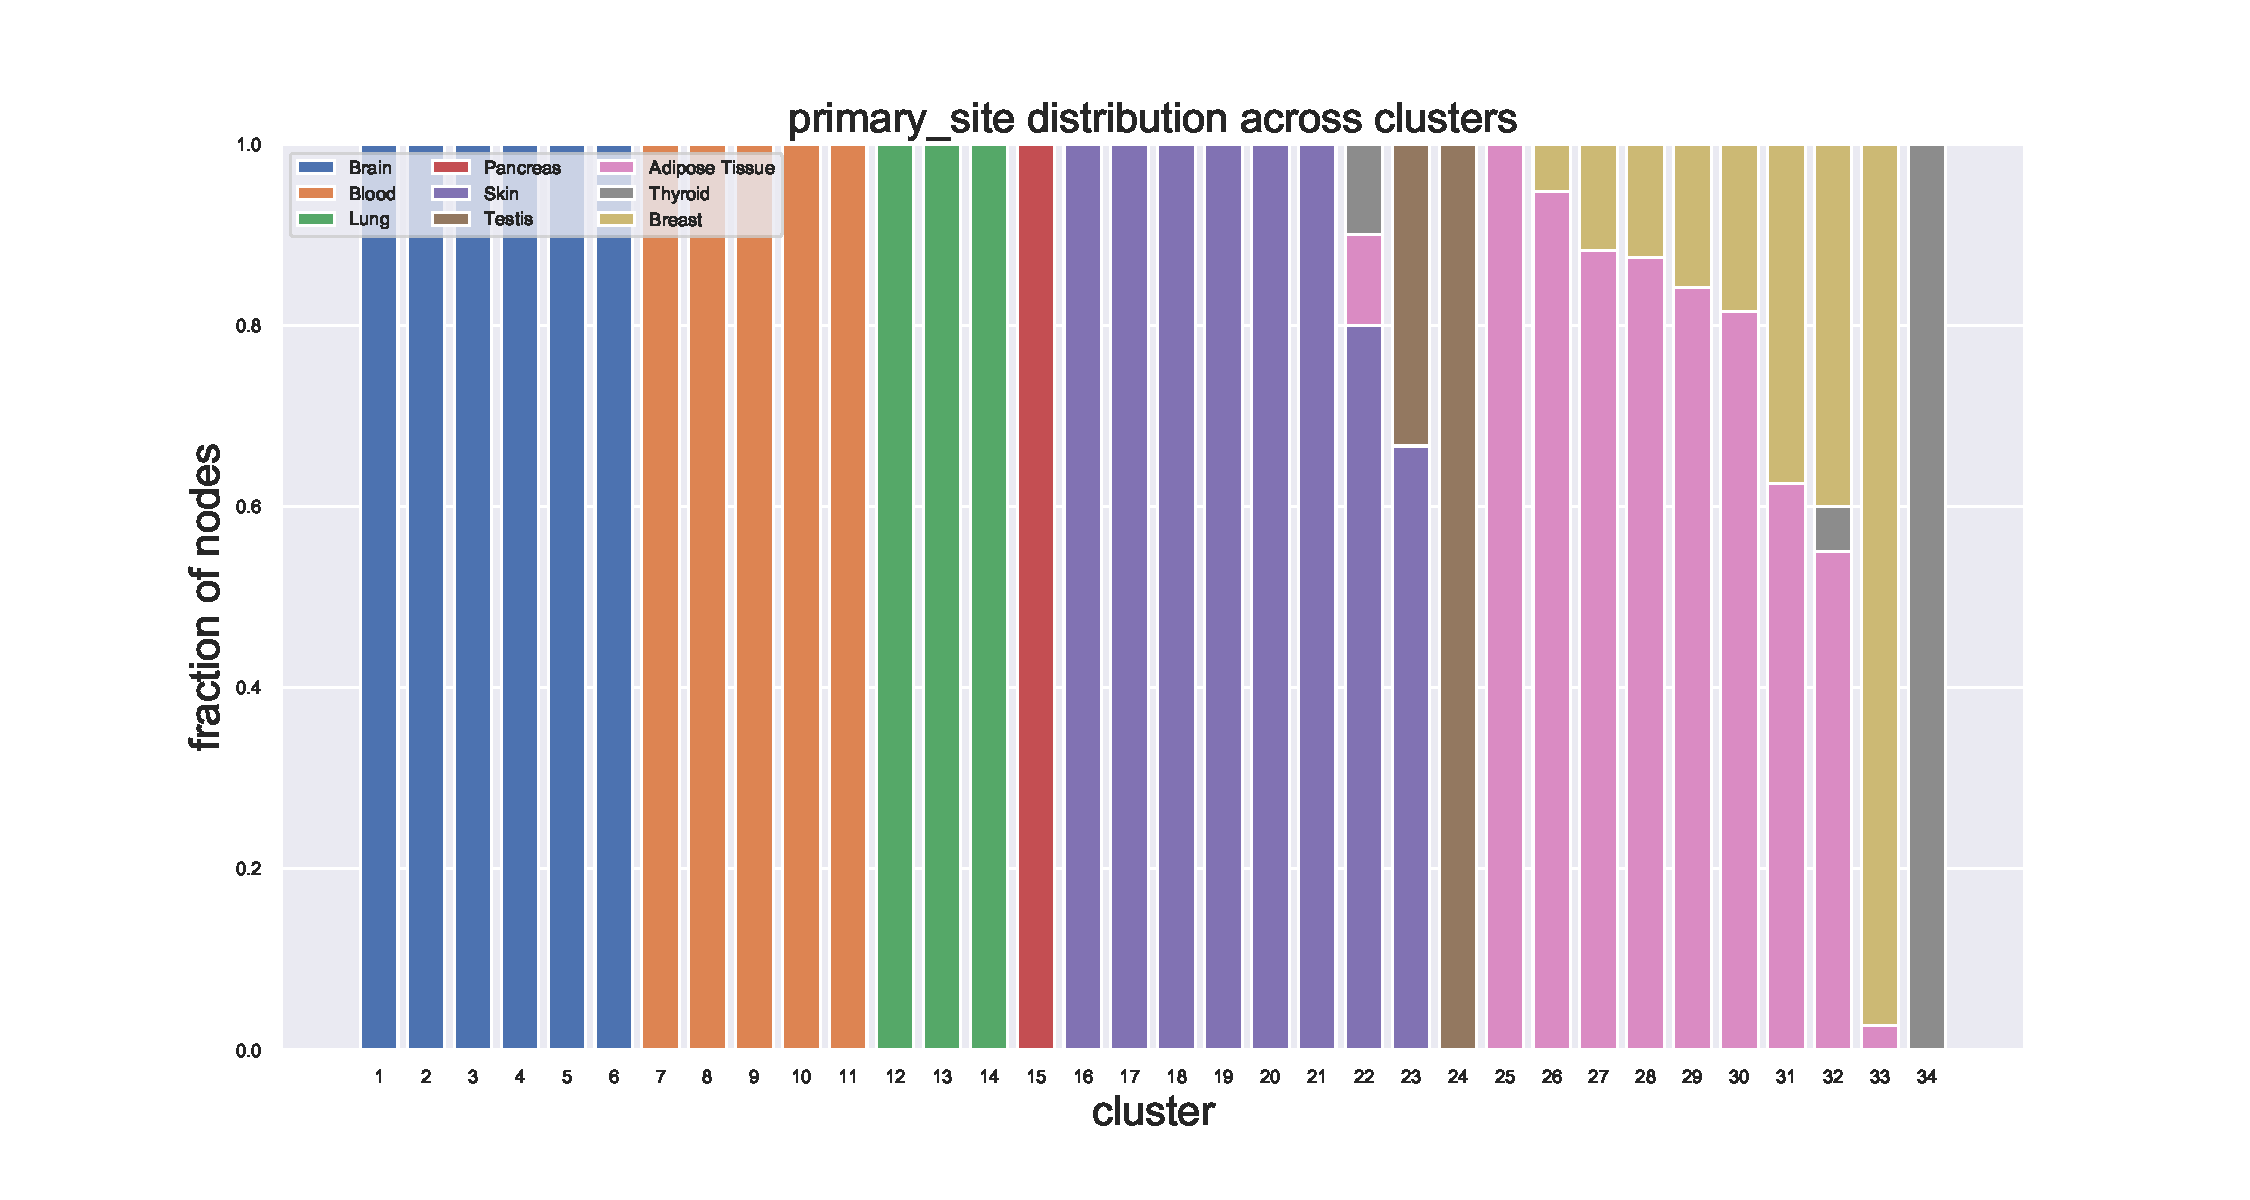
\includegraphics[width=0.9\linewidth]{pictures/topic/gtex/oversigma_10tissue/fraction_clustercomposition_l2_primary_site.pdf}
    \caption{Normalised composition of clusters at a deeper level.}
    \label{fig:topic/gtex/oversigma_10tissue/fraction_clustercomposition_l2_primary_site}
\end{figure}
Even looking at sub-tissues the results is quite good. It is not always easy to separate all the sub-parts of brain, nevertheless the cerebellum is well identified (column 13) and blood is distinguished in whole blood (columns 1-4) and lymphocytes (column 10).
\begin{figure}[htb!]
    \centering
    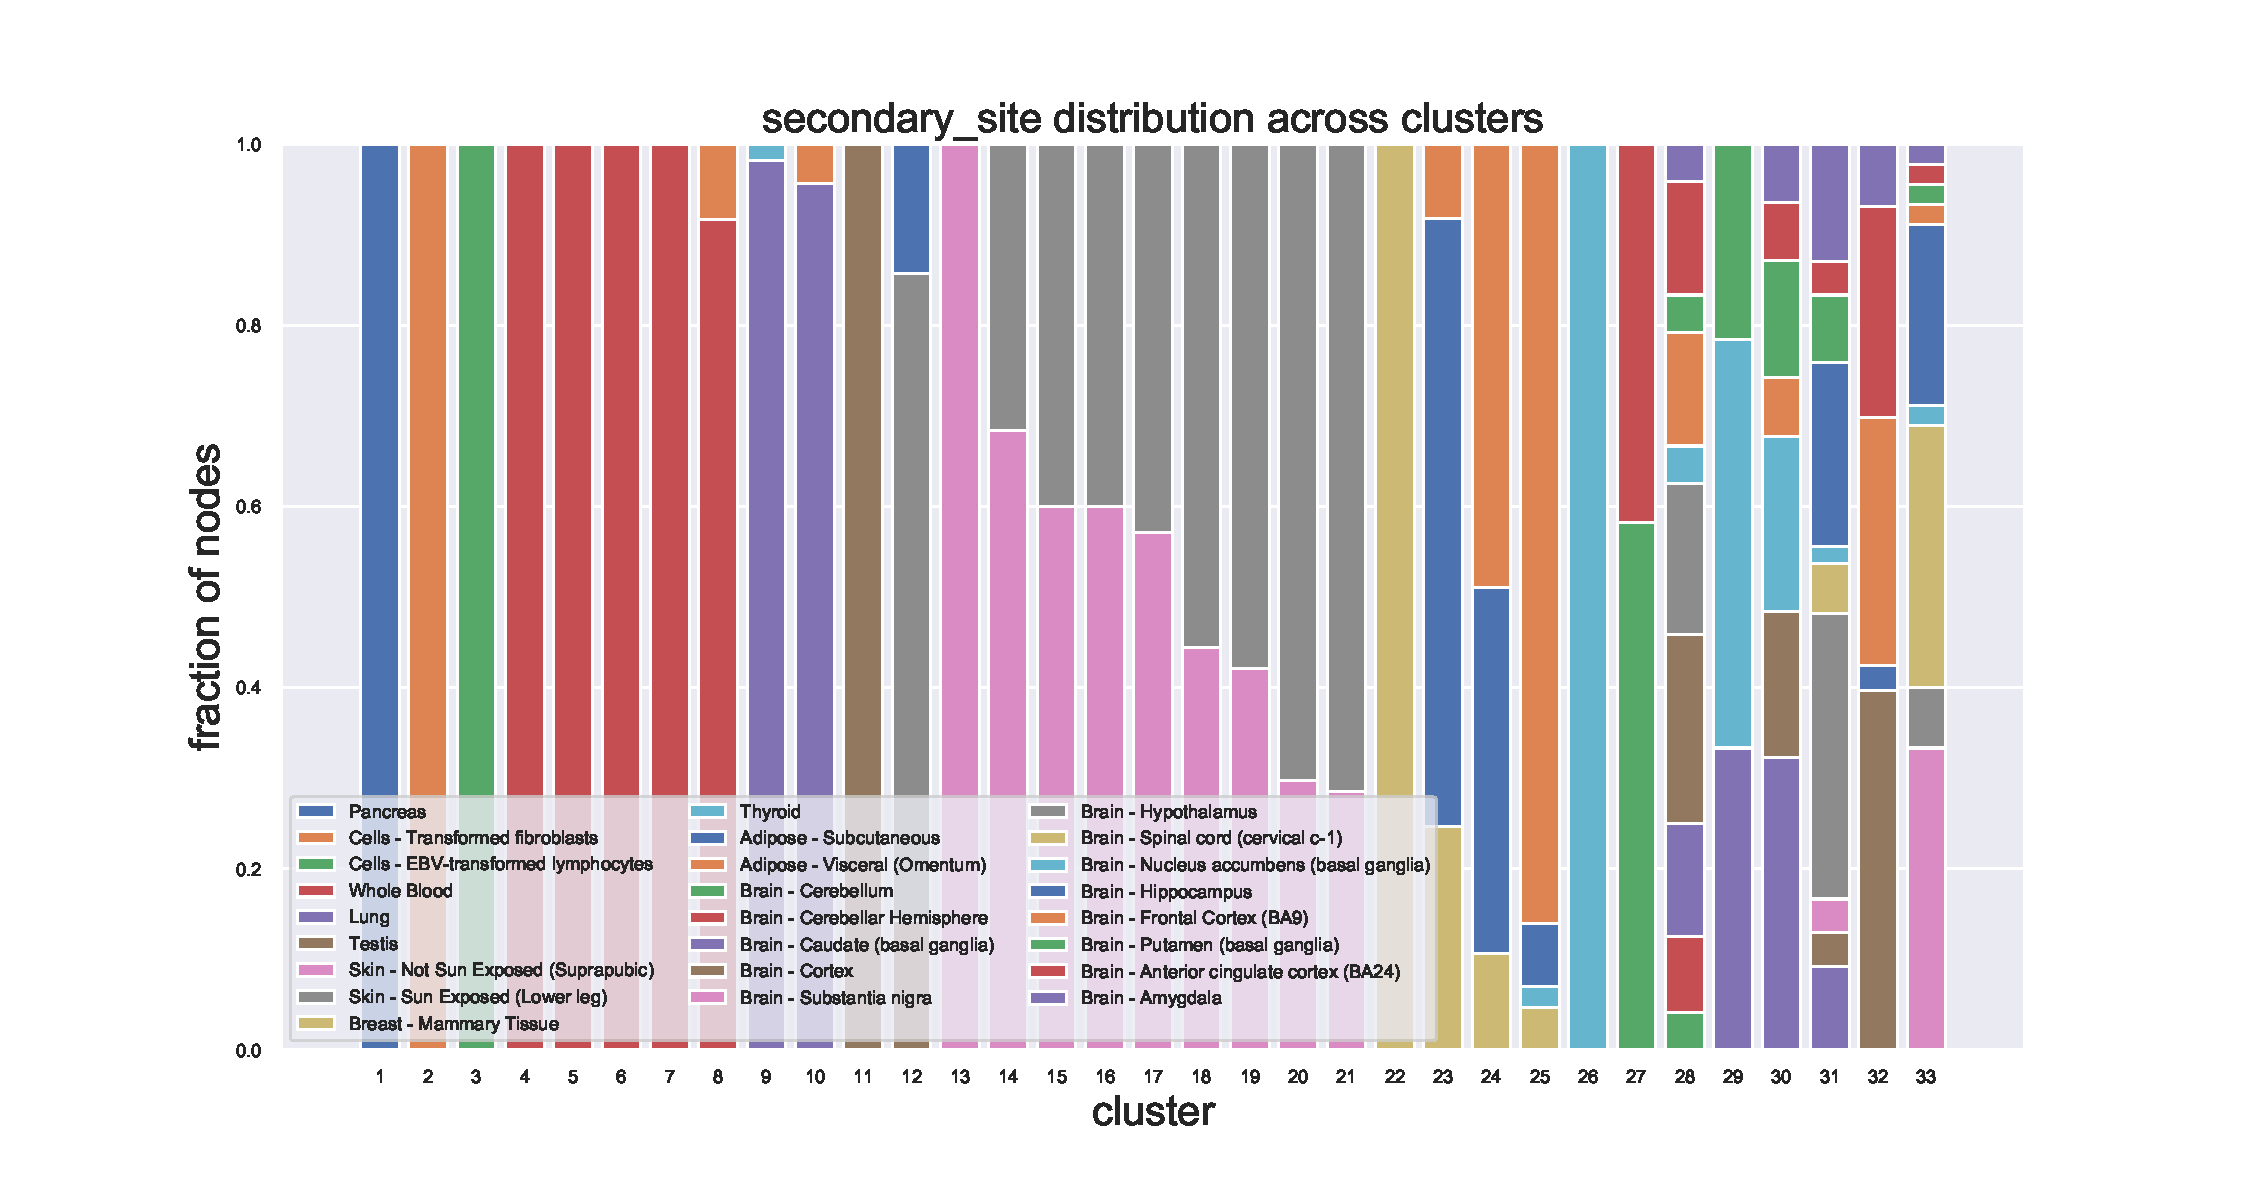
\includegraphics[width=0.9\linewidth]{pictures/topic/gtex/oversigma_10tissue/fraction_clustercomposition_l2_secondary_site.pdf}
    \caption{Normalised composition of clusters with respect to the secondary site subtissue labels.}
    \label{fig:topic/gtex/oversigma_10tissue/fraction_clustercomposition_l2_secondary_site}
\end{figure}

\subsection{Shuffling}
A null model of cluster composition is necessary In order to be able to state that a result is better than expected. This was done by doing the same analysis but reshuffling the labels of the nodes. Doing so the number of clusters and the cluster sizes are maintained. In figure~\ref{fig:topic/gtex/oversigma_10tissue/shuffledclustercomposition_l3_primary_site} an example of clustering with random labels, it is evident that all clusters have similar and homogeneous composition. Note that not every tissue has the same number of samples, so for example blood is more represented than other tissues.
\begin{figure}[htb!]
	\centering
	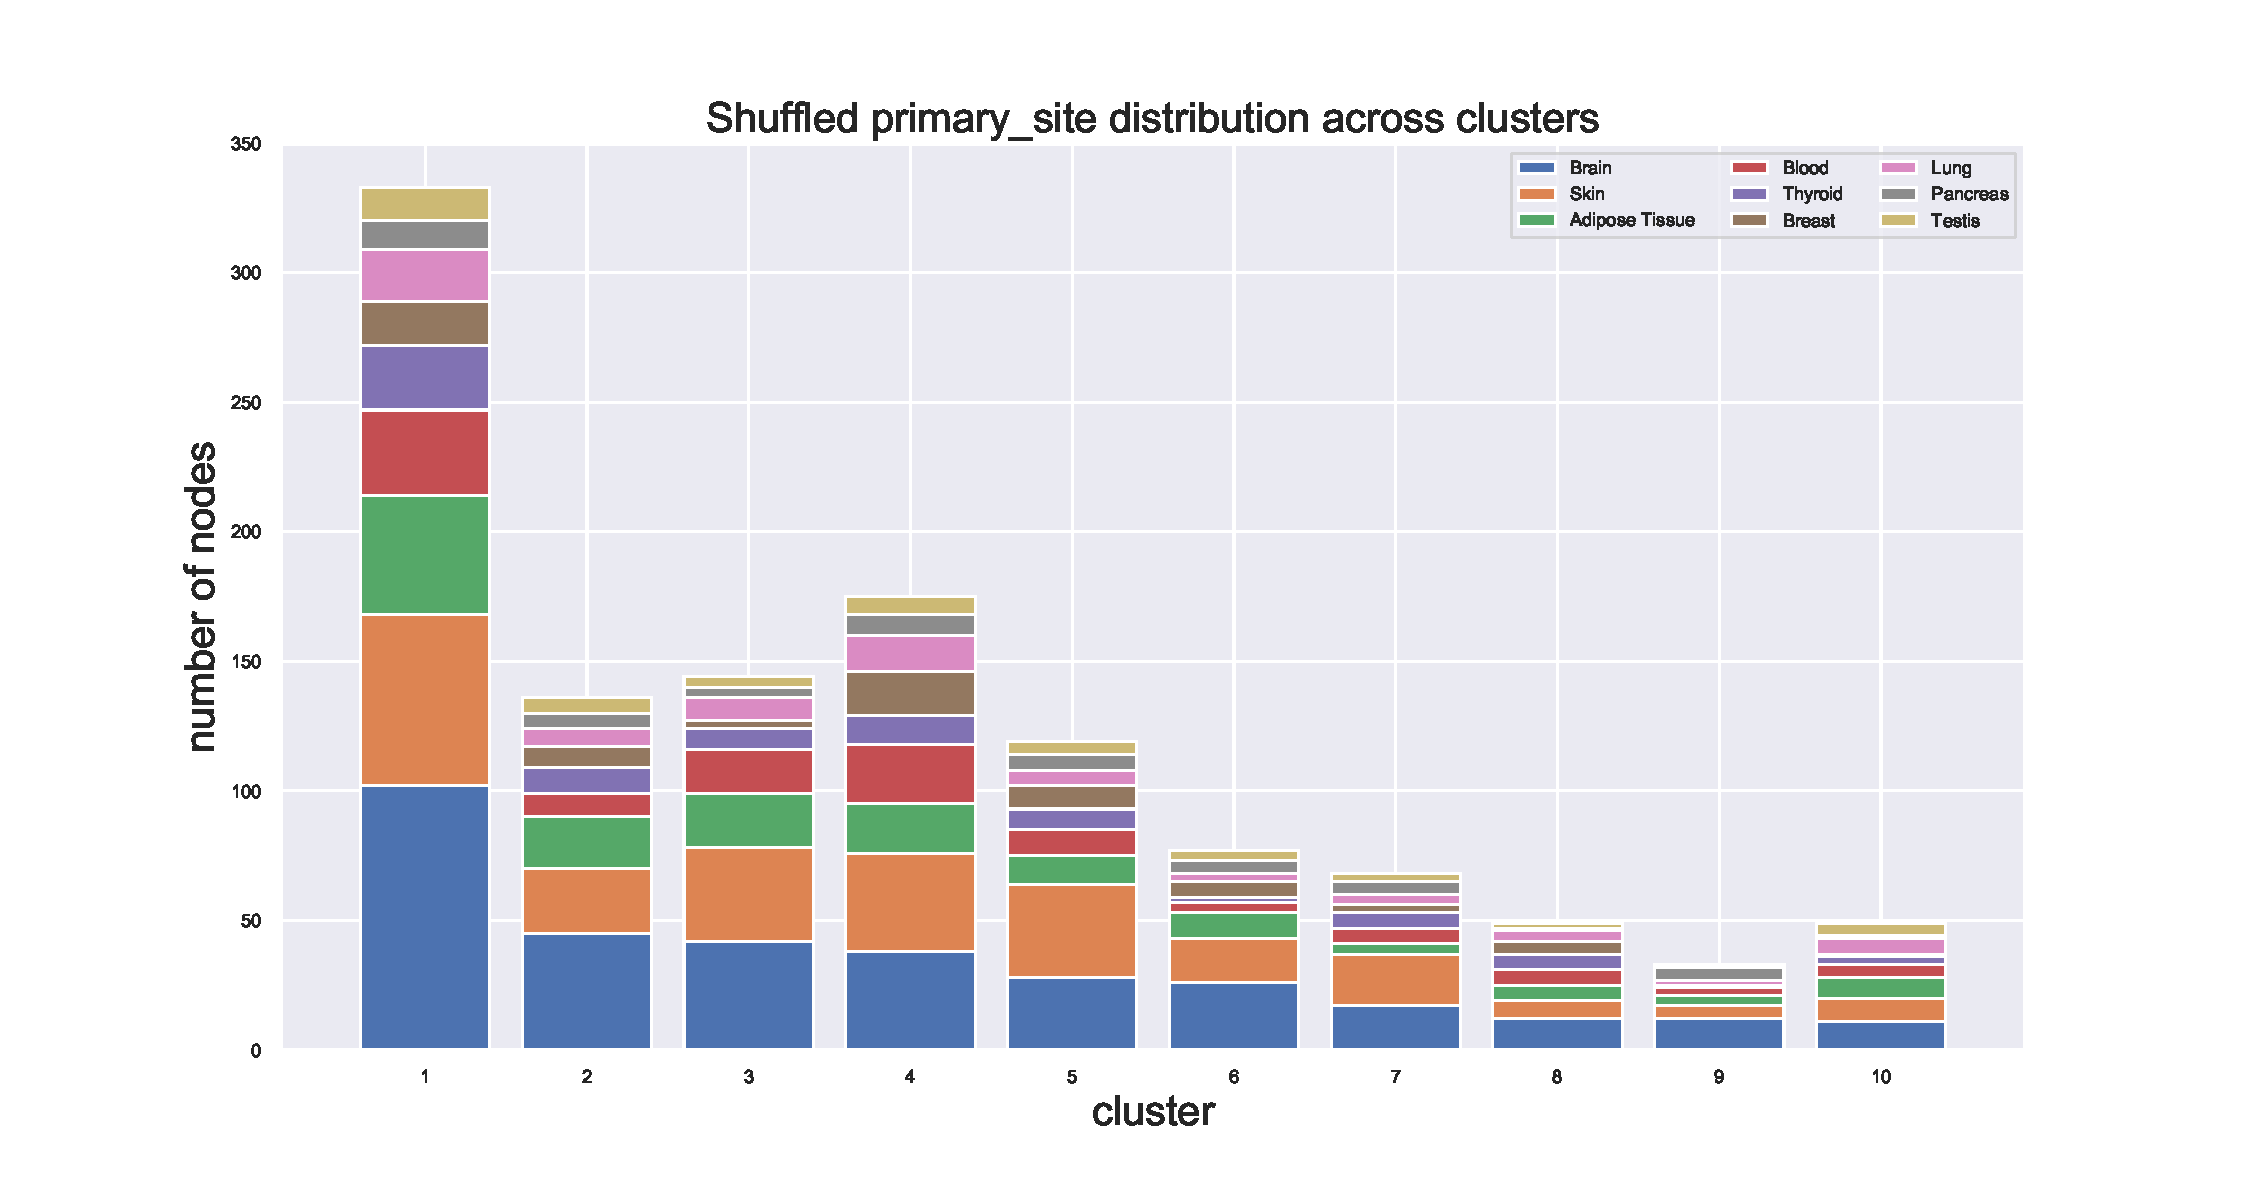
\includegraphics[width=0.8\linewidth]{pictures/topic/gtex/oversigma_10tissue/shuffledclustercomposition_l3_primary_site}
	\caption{Example of visualization of clusters with reshuffled labels.}
	\label{fig:topic/gtex/oversigma_10tissue/shuffledclustercomposition_l3_primary_site}
\end{figure}

All the results described in the previous pictures are quite qualitative. To have a more objective and mathematical measure of the success of the algorithm it is possible to measure the fraction of the most representative label in each cluster $k$
\[
max_{l\in labels}\left(\frac{n_{l k}}{n_k}\right)
\]
with $n_{l k}$ is the numbers of nodes labeled $l$ in cluster $k$ and $n_k$ is the number of nodes in cluster $k$. This is represented in figure~\ref{fig:gtex/oversigma_10tissue/shuffledcluster_maximum_l2_primary_site} for the level where the V-measure is maximized (best results are expected here). In figure~\ref{fig:gtex/oversigma_10tissue/shuffledcluster_maximum_l2_primary_site} on the left is shown the most representative label fraction versus for each cluster, on the right the histograms of the same quantity. It is evident that models' clusters are very homogeneous with the majority of cluster with almost $100\%$ of the same tissue. It is also clear that reshuffling the labels the result is very different and so the models behave better than expected. 
\begin{figure}[htb!]
    \centering
    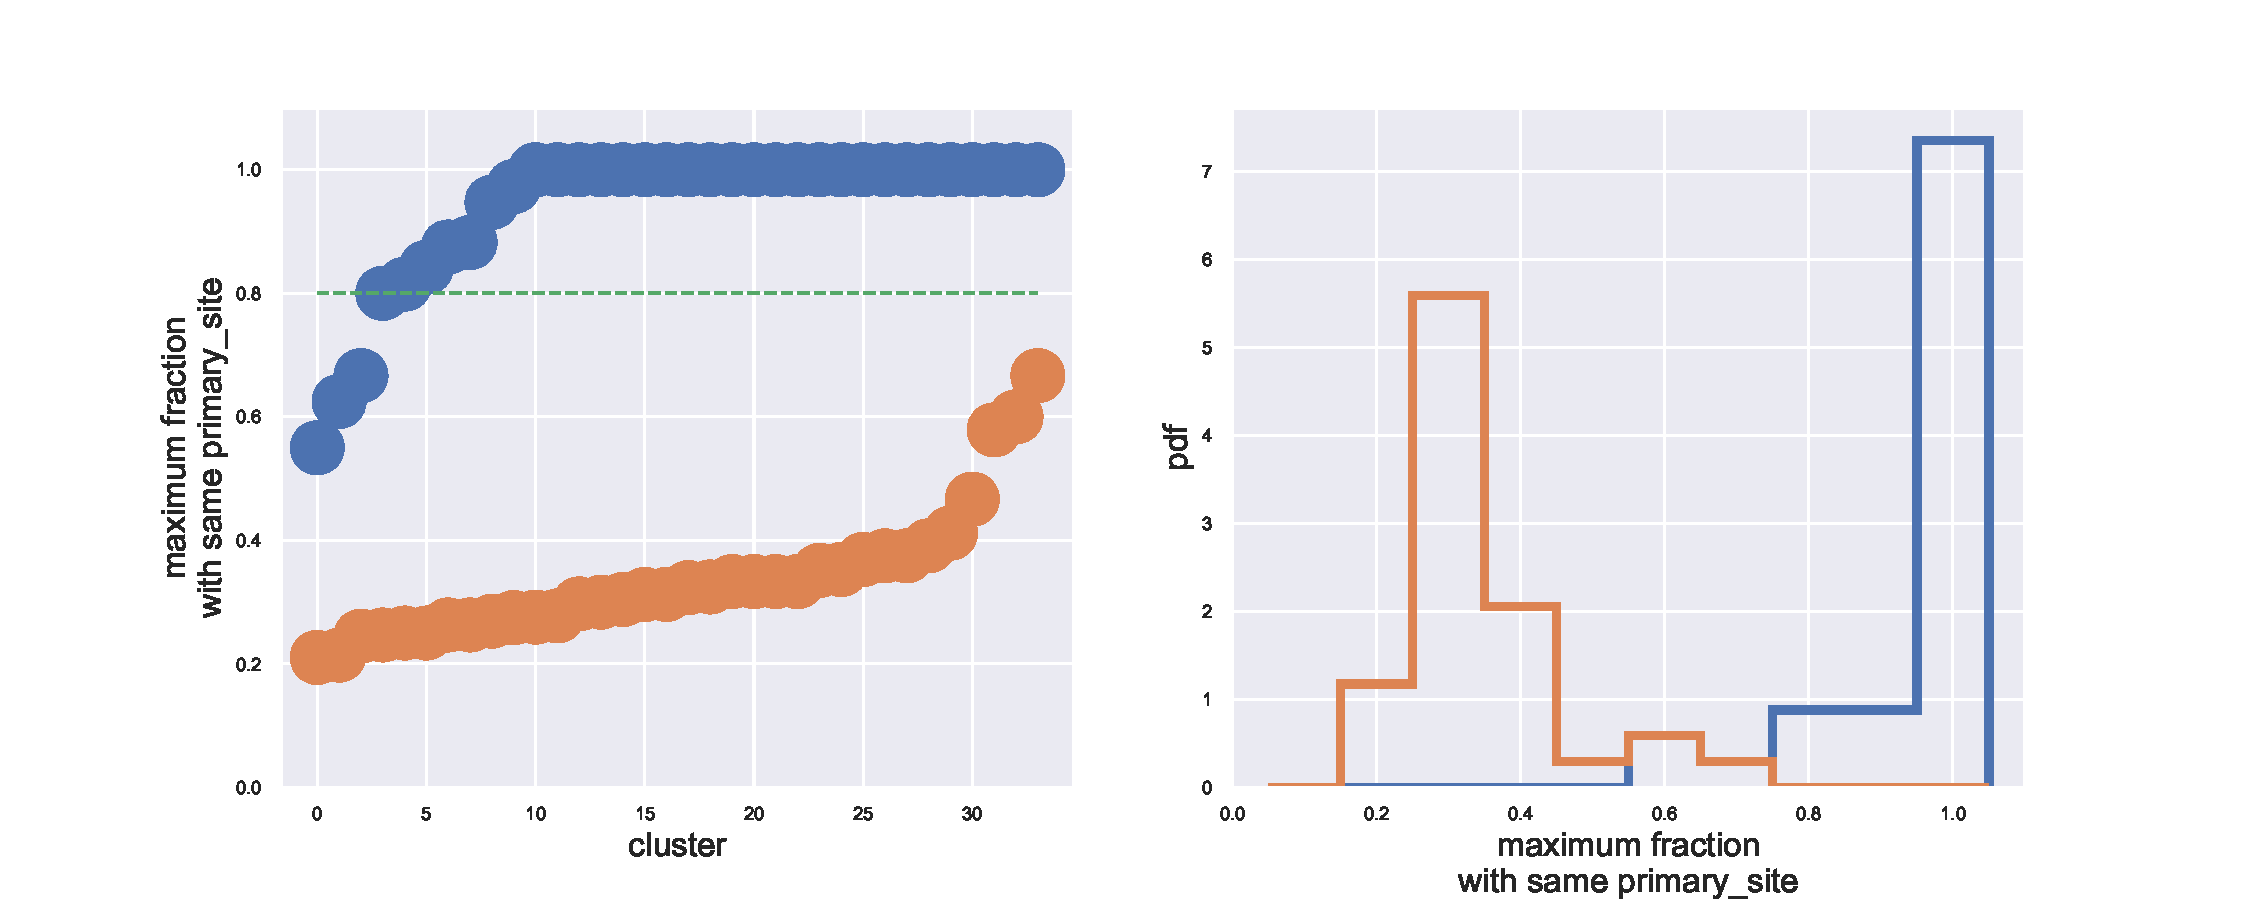
\includegraphics[width=0.9\linewidth]{pictures/topic/gtex/oversigma_10tissue/shuffledcluster_maximum_l2_primary_site.pdf}
    \caption{Most representative label versus cluster size.}
    \label{fig:gtex/oversigma_10tissue/shuffledcluster_maximum_l2_primary_site}
\end{figure}
In figure~\ref{fig:topic/gtex/oversigma_10tissue/shuffledcluster_maximum*} the same analysis is done for every level of the hierarchy. It is interesting to notice that at deeper levels (upper left in the figure) the random reshuffling and the real labels have the same behavior. This is due to the fact that at this level clusters are very small and so it is easier to pick up nodes with the same level (in the extreme case of a cluster with size 1 it is always full with the same label). This shows that the deeper level it is not interesting, results are exactly the same with random labels;  moreover the reshuffling null model it is good to show up eventual biases due to small cluster sizes.
\begin{figure}[htb!]
    \centering
    \begin{minipage}{0.45\textwidth}
    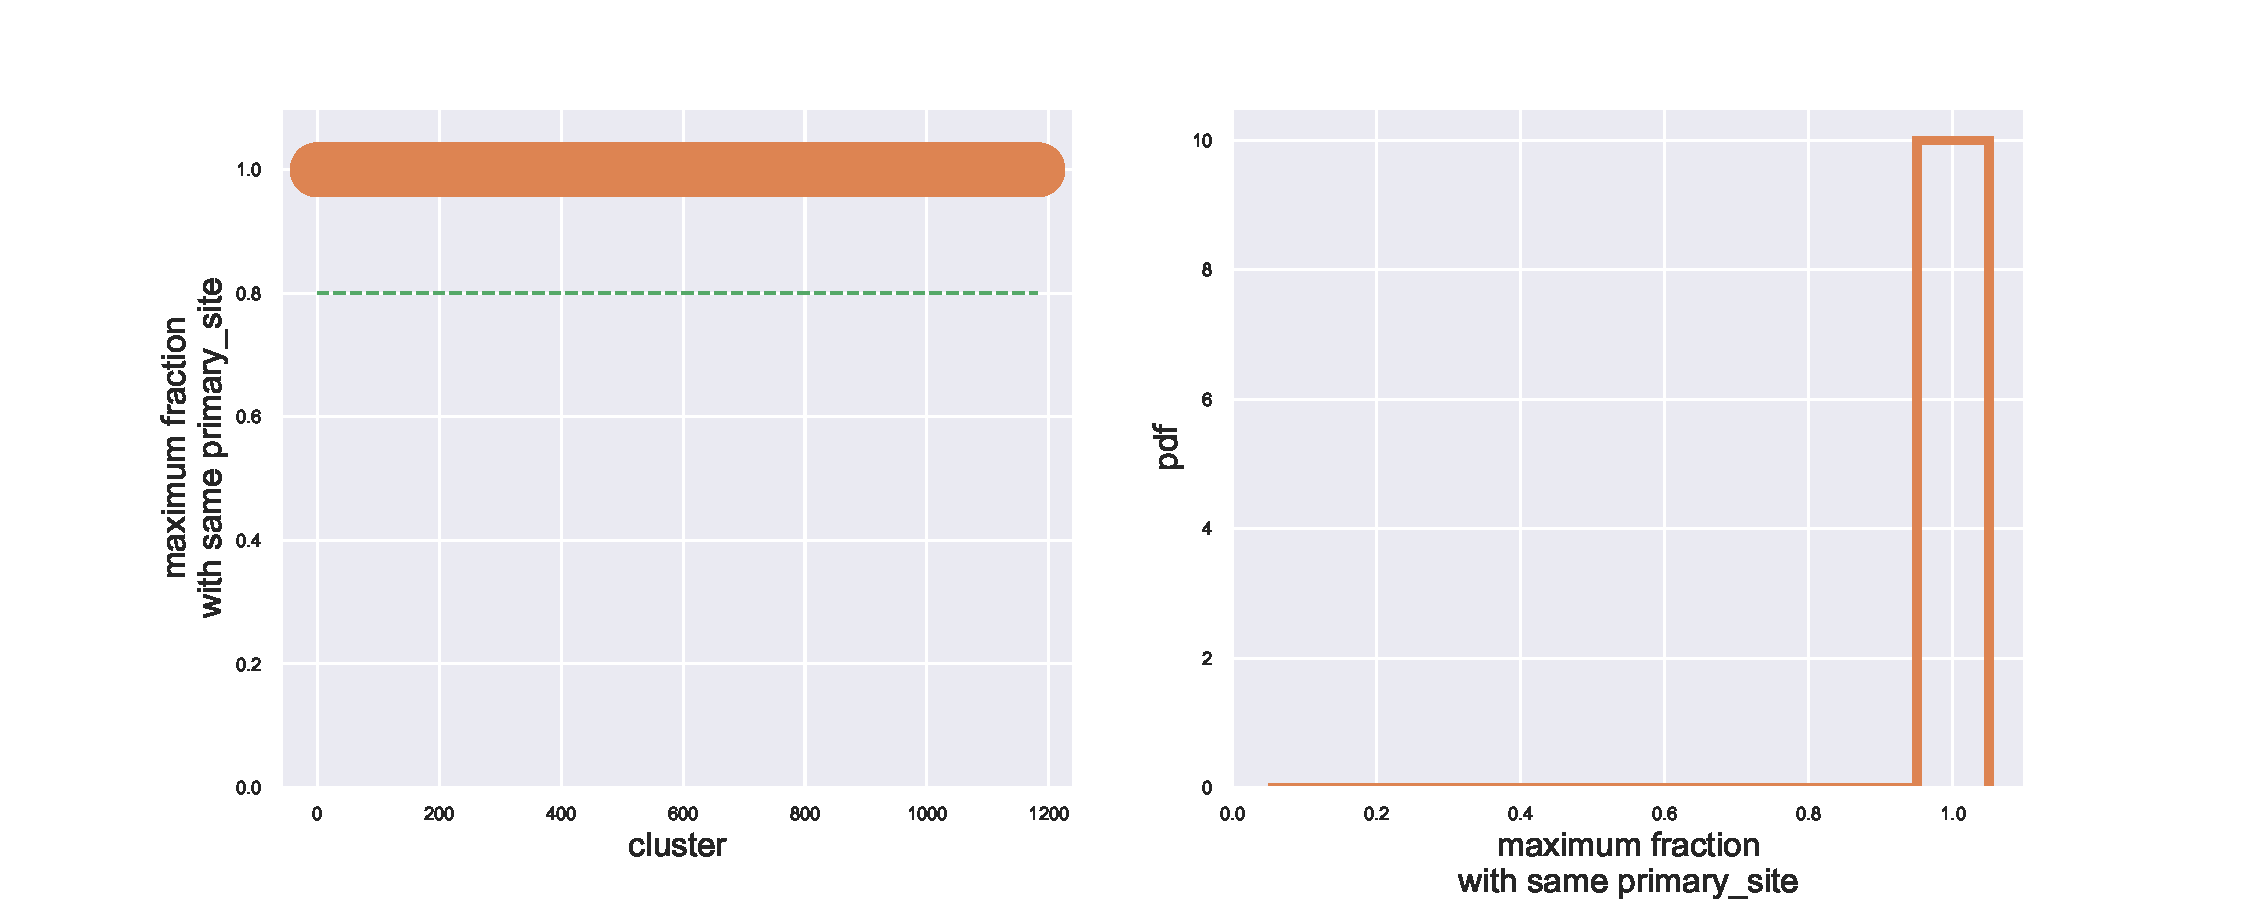
\includegraphics[width=0.9\linewidth]{pictures/topic/gtex/oversigma_10tissue/shuffledcluster_maximum_l0_primary_site.pdf}
    \end{minipage}
    \hspace{3mm}
    \begin{minipage}{0.45\textwidth}
    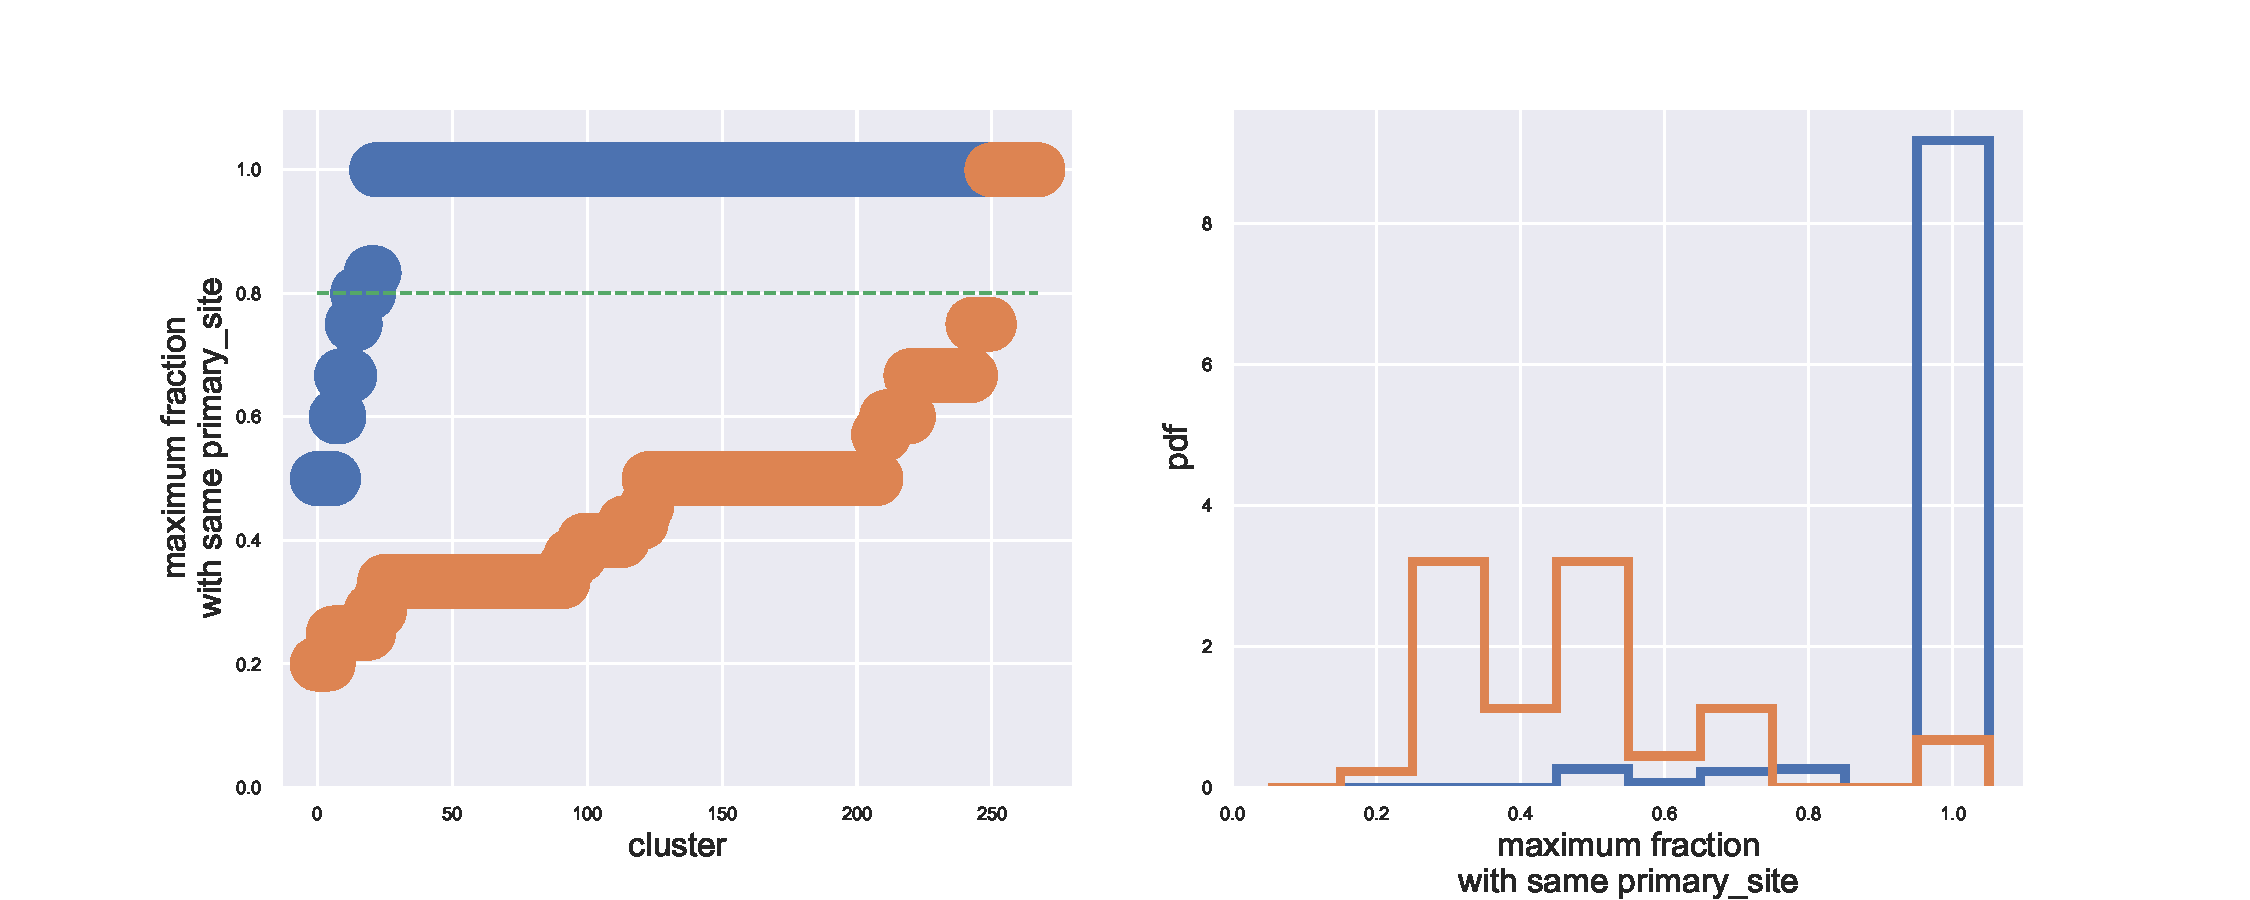
\includegraphics[width=0.9\linewidth]{pictures/topic/gtex/oversigma_10tissue/shuffledcluster_maximum_l1_primary_site.pdf}
    \end{minipage}
    \\
    \begin{minipage}{0.45\textwidth}
    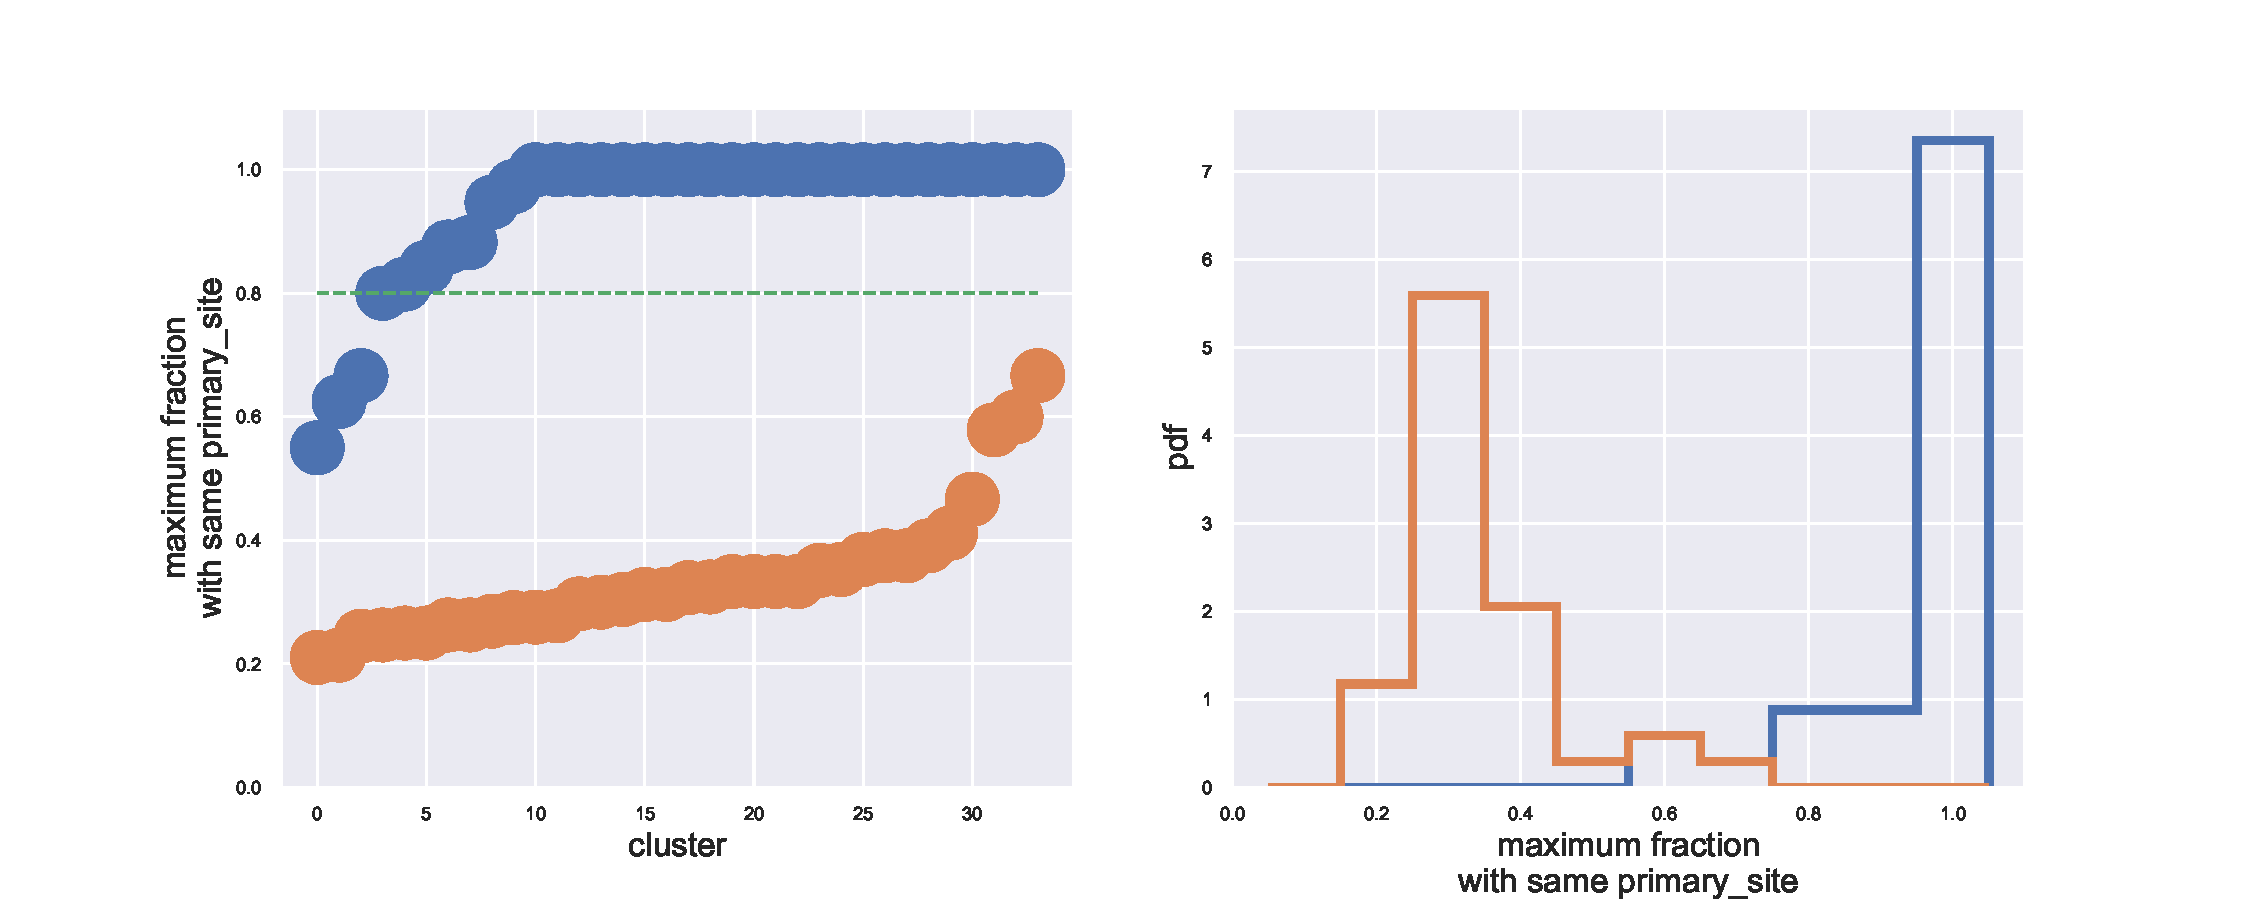
\includegraphics[width=0.9\linewidth]{pictures/topic/gtex/oversigma_10tissue/shuffledcluster_maximum_l2_primary_site.pdf}
    \end{minipage}
    \hspace{3mm}
    \begin{minipage}{0.45\textwidth}
    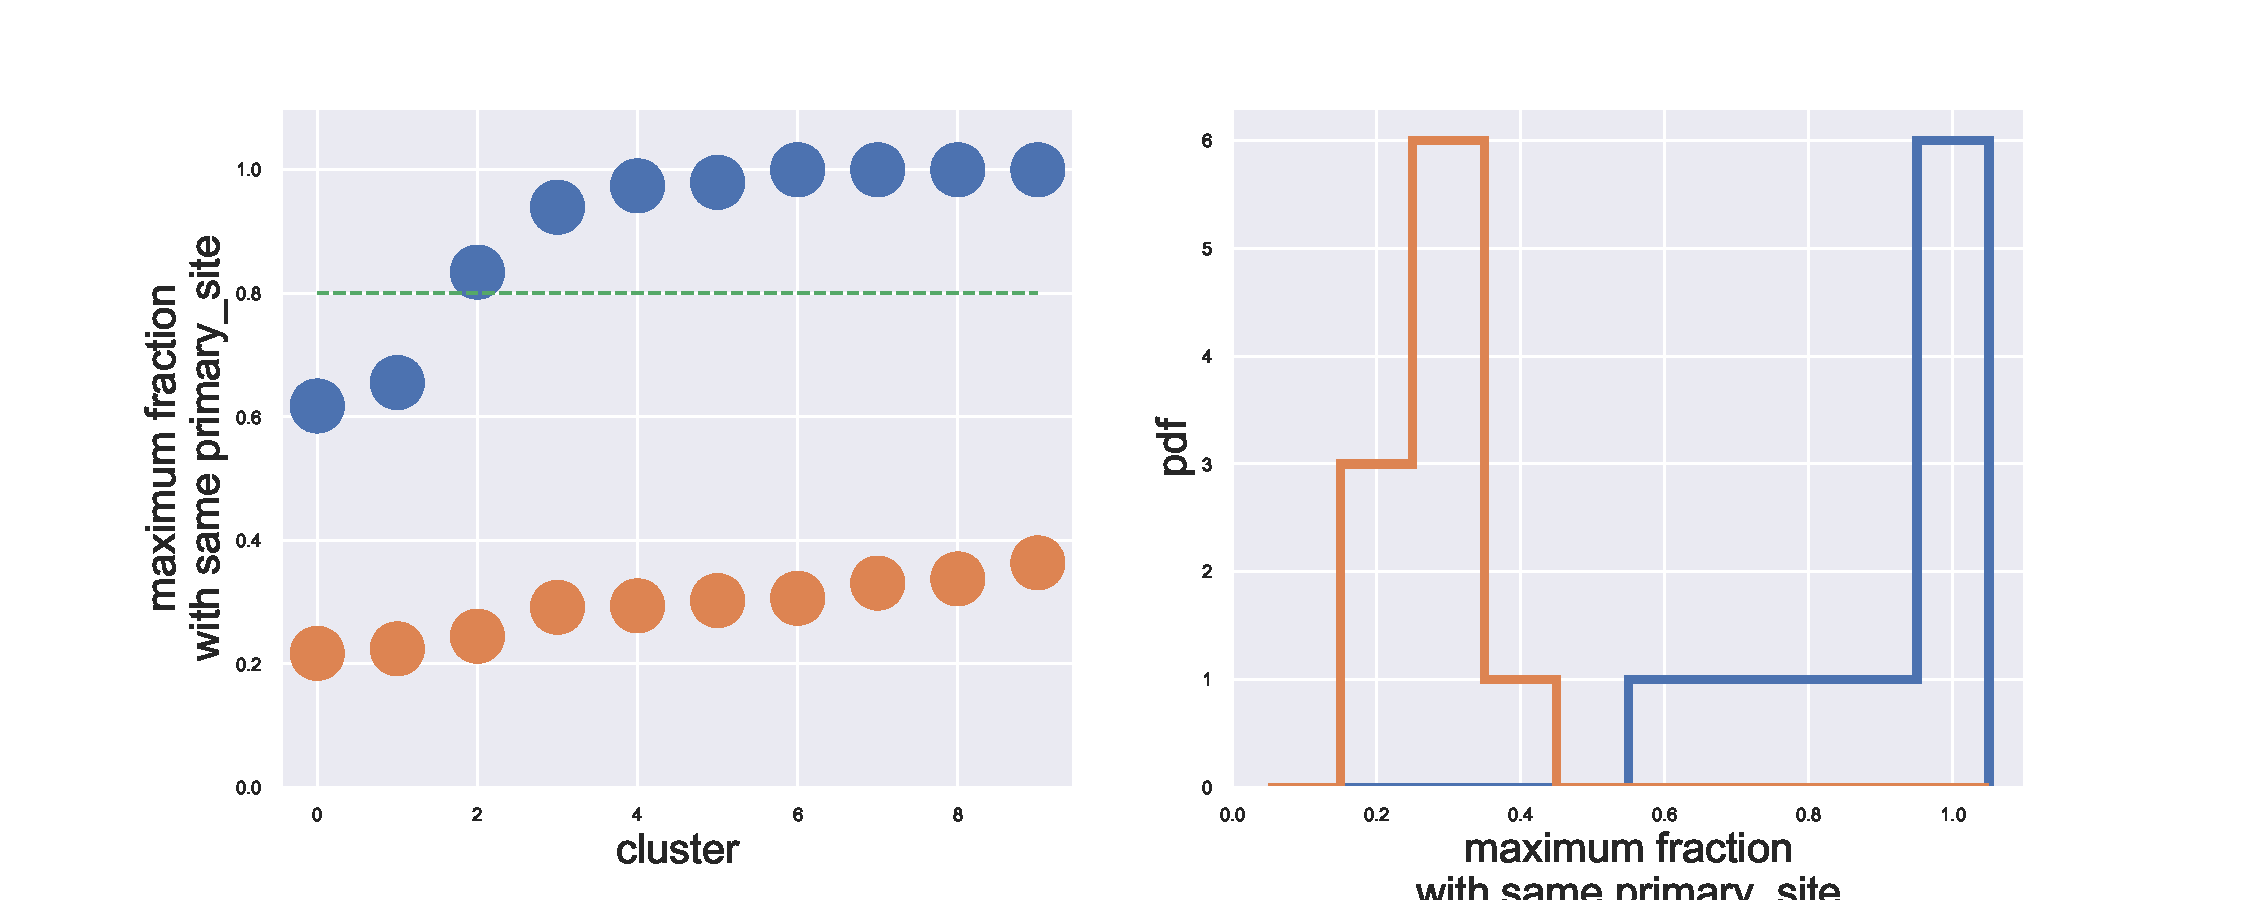
\includegraphics[width=0.9\linewidth]{pictures/topic/gtex/oversigma_10tissue/shuffledcluster_maximum_l3_primary_site.pdf}
    \end{minipage}
    \caption{Fraction of the most representative label in all clusters for different levels of the hierarchy. From upper left the deeper layer than down right the upper one.}
    \label{fig:topic/gtex/oversigma_10tissue/shuffledcluster_maximum*}
\end{figure}

A similar analysis can be made considering not just the number of the cluster but the cluster size, this is shown in figure~\ref{fig:topic/gtex/oversigma_10tissue/shuffledclusterhomosize_l3_primary_site}. It is interesting to notice that the shuffle null model and the real labels clusters are evidently different, so there must be some kind of signal. It is clear that the model is able to output big clusters full with the same label.
\begin{figure}[htb!]
	\centering
	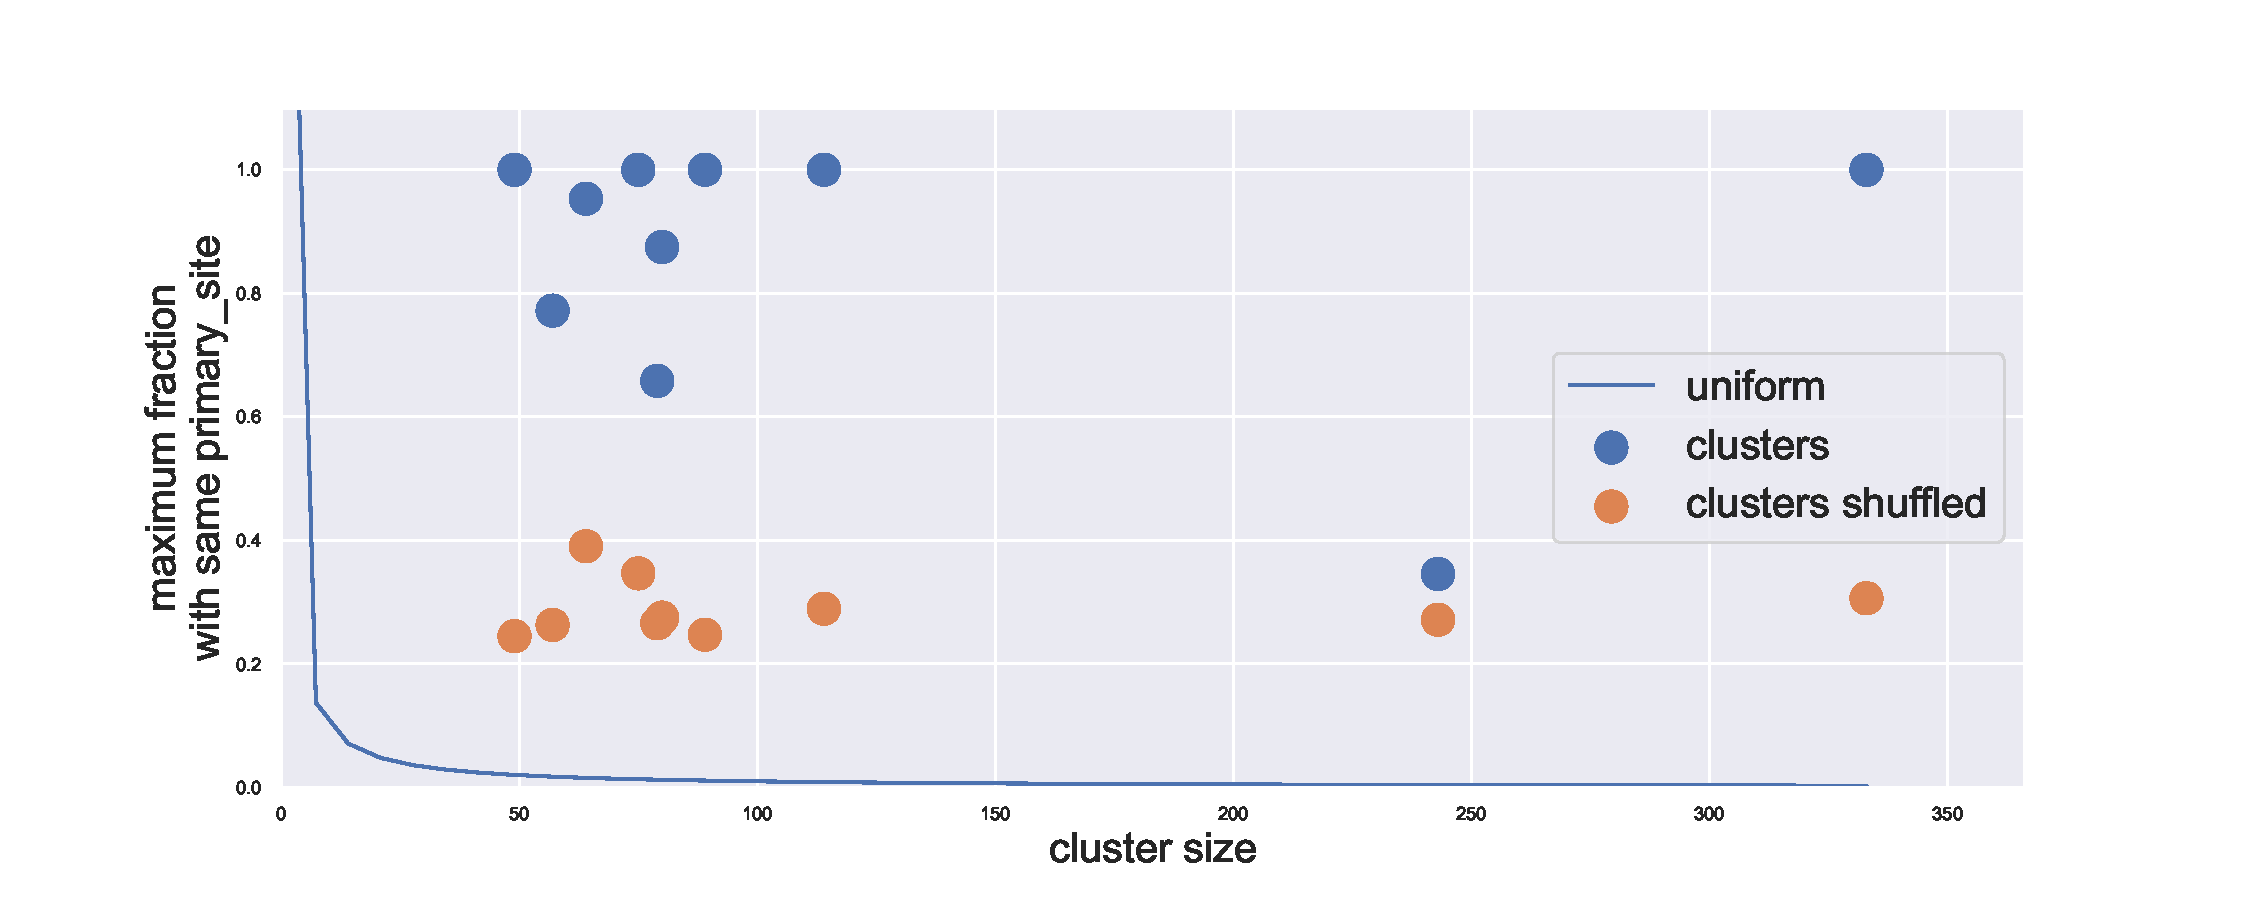
\includegraphics[width=0.9\linewidth]{pictures/topic/gtex/oversigma_10tissue/shuffledclusterhomosize_l3_primary_site.pdf}
	\caption{Fraction of most representative label versus cluster size.}
	\label{fig:topic/gtex/oversigma_10tissue/shuffledclusterhomosize_l3_primary_site}
\end{figure}
In figure~\ref{fig:topic/gtex/oversigma_10tissue/shuffledclusterhomosize_l*} the same analysis for  all the levels of the hierarchy. It is interesting to see how going up in the hierarchy the two signals become different, as shown before the deeper layer (upper left in the image) is not different from null model and so it is not interesting.
\begin{figure}[htb!]
	\centering
	\begin{minipage}{0.45\textwidth}
		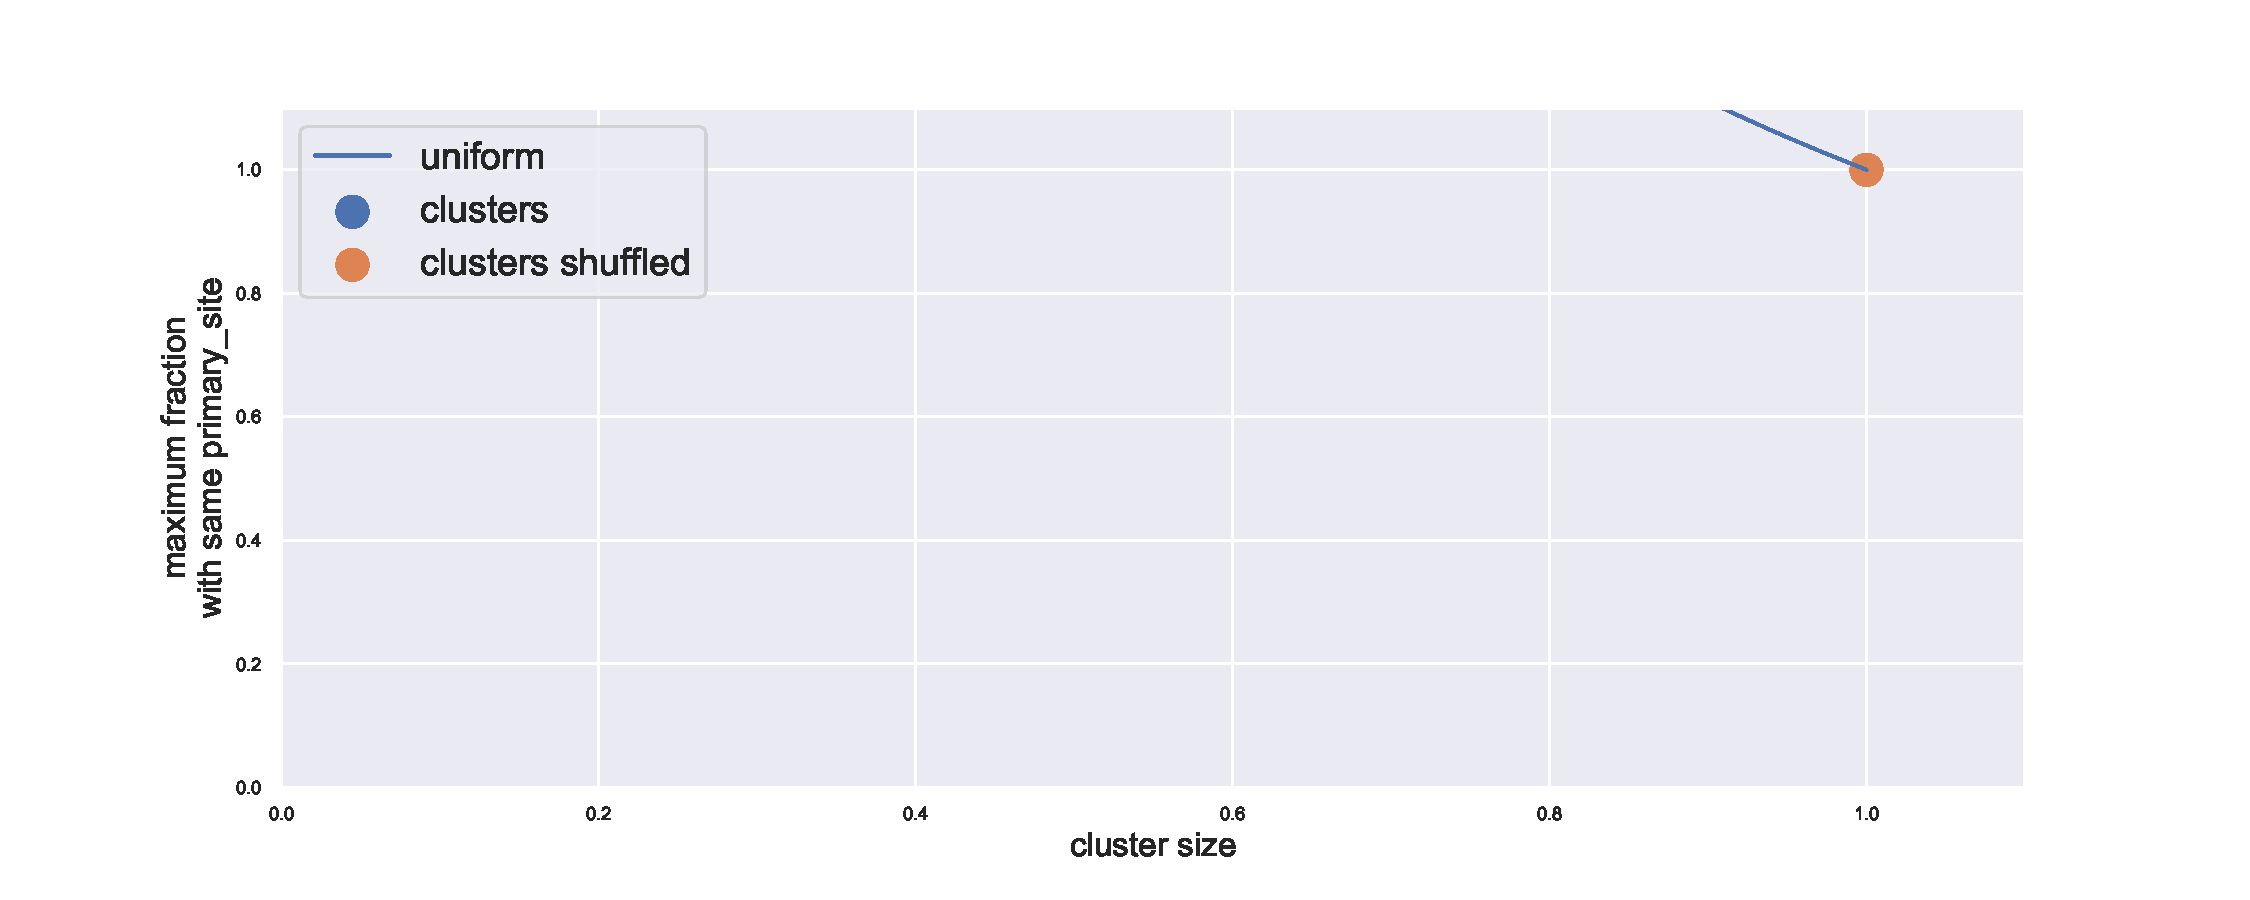
\includegraphics[width=0.9\linewidth]{pictures/topic/gtex/oversigma_10tissue/shuffledclusterhomosize_l0_primary_site.pdf}
	\end{minipage}
	\hspace{3mm}
	\begin{minipage}{0.45\textwidth}
		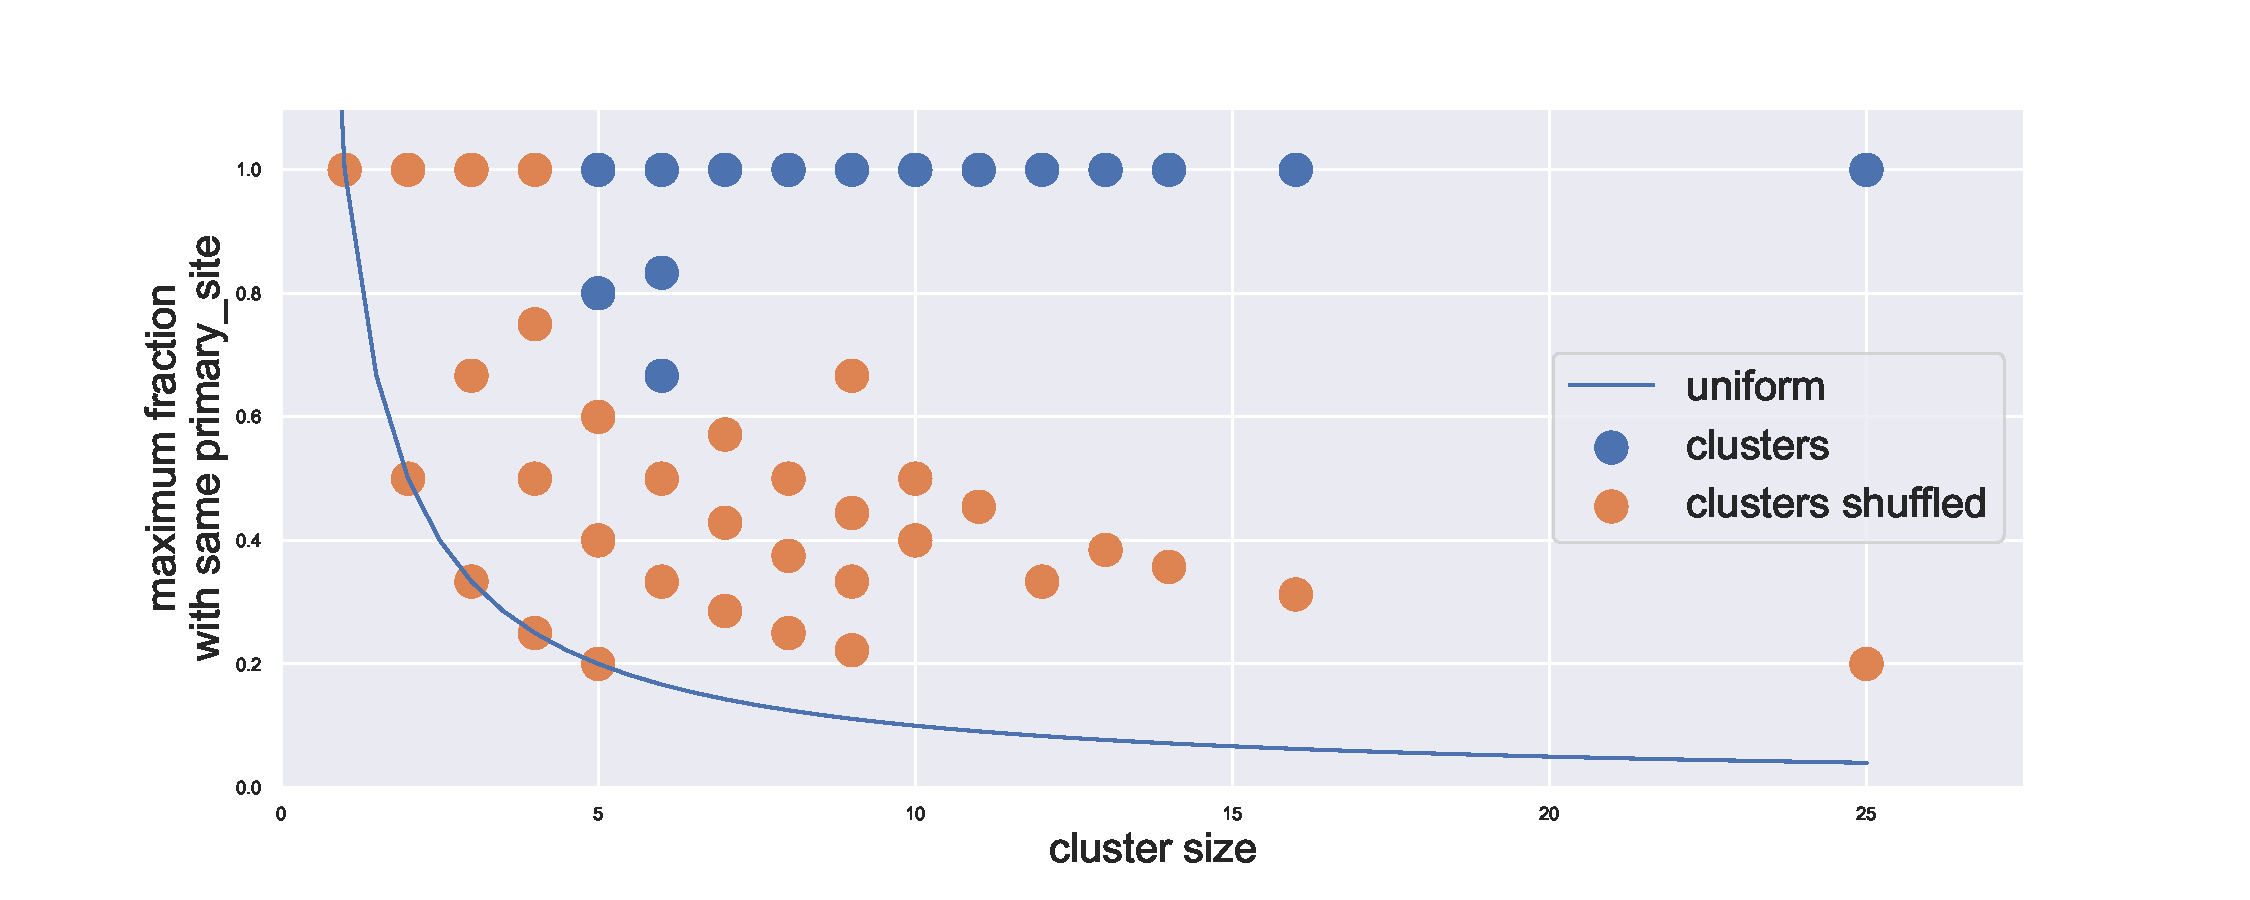
\includegraphics[width=0.9\linewidth]{pictures/topic/gtex/oversigma_10tissue/shuffledclusterhomosize_l1_primary_site.pdf}
	\end{minipage}
	\\
	\begin{minipage}{0.45\textwidth}
		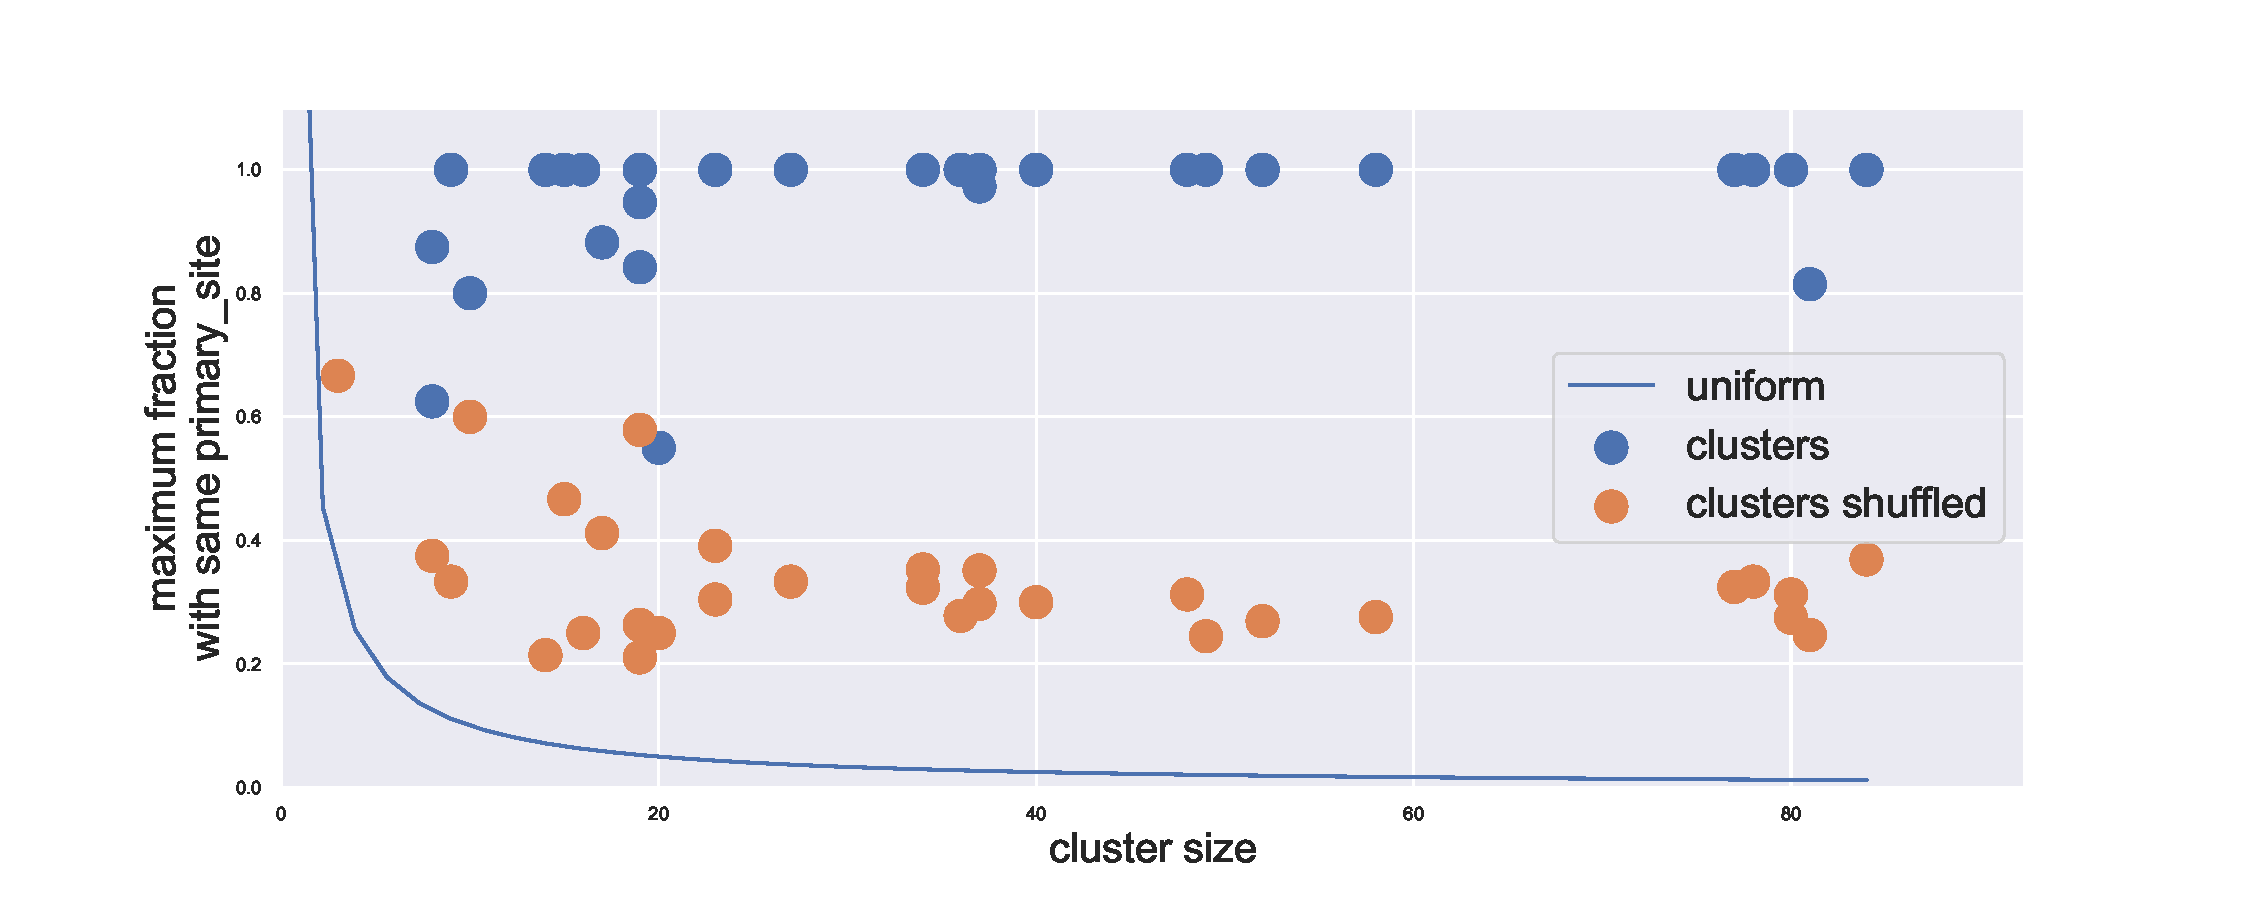
\includegraphics[width=0.9\linewidth]{pictures/topic/gtex/oversigma_10tissue/shuffledclusterhomosize_l2_primary_site.pdf}
	\end{minipage}
	\hspace{3mm}
	\begin{minipage}{0.45\textwidth}
		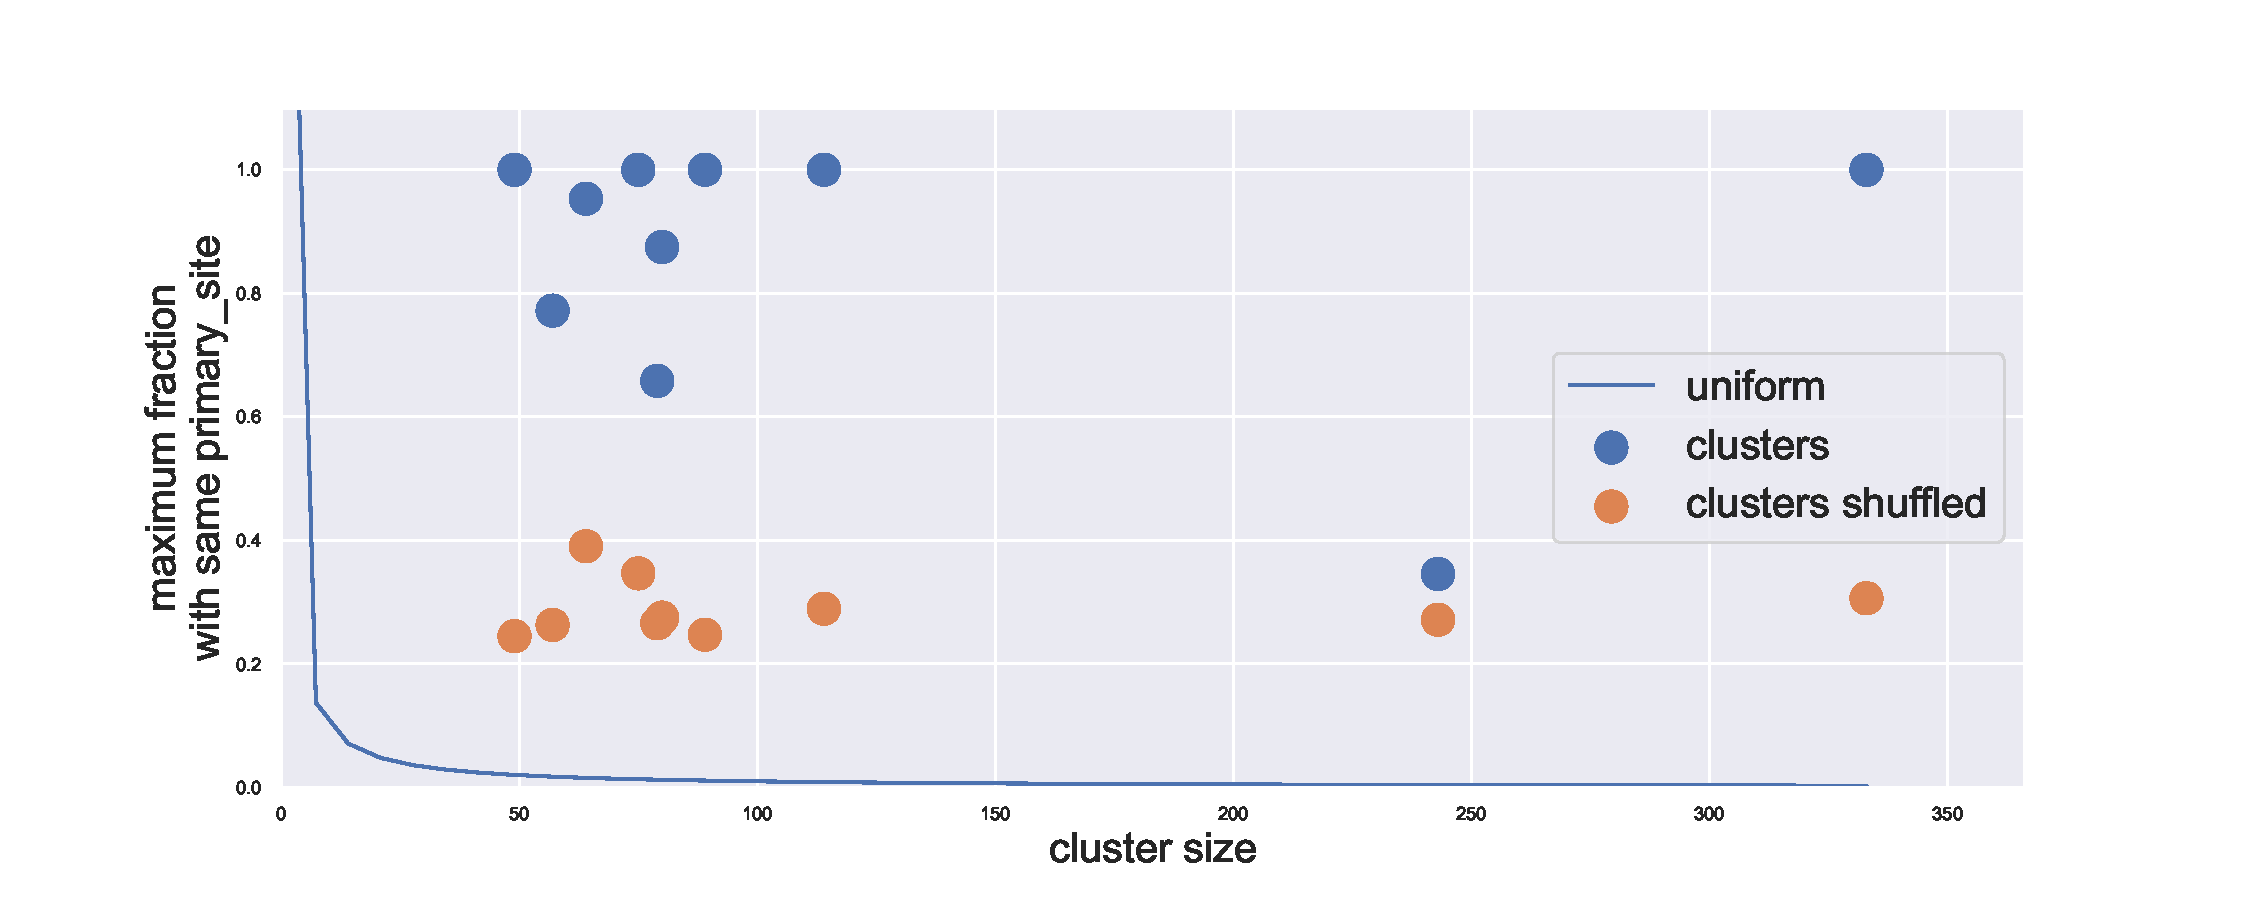
\includegraphics[width=0.9\linewidth]{pictures/topic/gtex/oversigma_10tissue/shuffledclusterhomosize_l3_primary_site.pdf}
	\end{minipage}
	\caption{Fraction of most representative label versus cluster size across the hierarchy. From upper left the deeper layer than down right the upper one.}
	\label{fig:topic/gtex/oversigma_10tissue/shuffledclusterhomosize_l*}
\end{figure}


At this point to deepen investigate the structure of the clusters it can be interesting to study how many labels are present in each cluster. In fact the fraction of most represented label defined above carries no information of what happens to the non most representative labels. For example if one cluster is composed of $80\%$ by label \textbf{A} and $20\%$ by label \textbf{B} and another cluster is composed $80\%$ by label \textbf{A}, $10\%$ by label \textbf{B} and $10\%$ by label \textbf{C} they have both fraction of maximum representative label $80\%$ but the second in this example is more heterogeneous. Counting the number of different labels in each cluster can reveal this sort of effects. In figure~\ref{fig:topic/gtex/oversigma_10tissue/shuffledcluster_shuffle_label_size_l3_primary_site} it is represented the number of different labels versus cluster size. It is evident that the reshuffling case is quite different from the real one, almost every cluster in the null model has got every label. It is interesting to notice that the model outputs even big cluster with one label.
\begin{figure}[htb!]
    \centering
    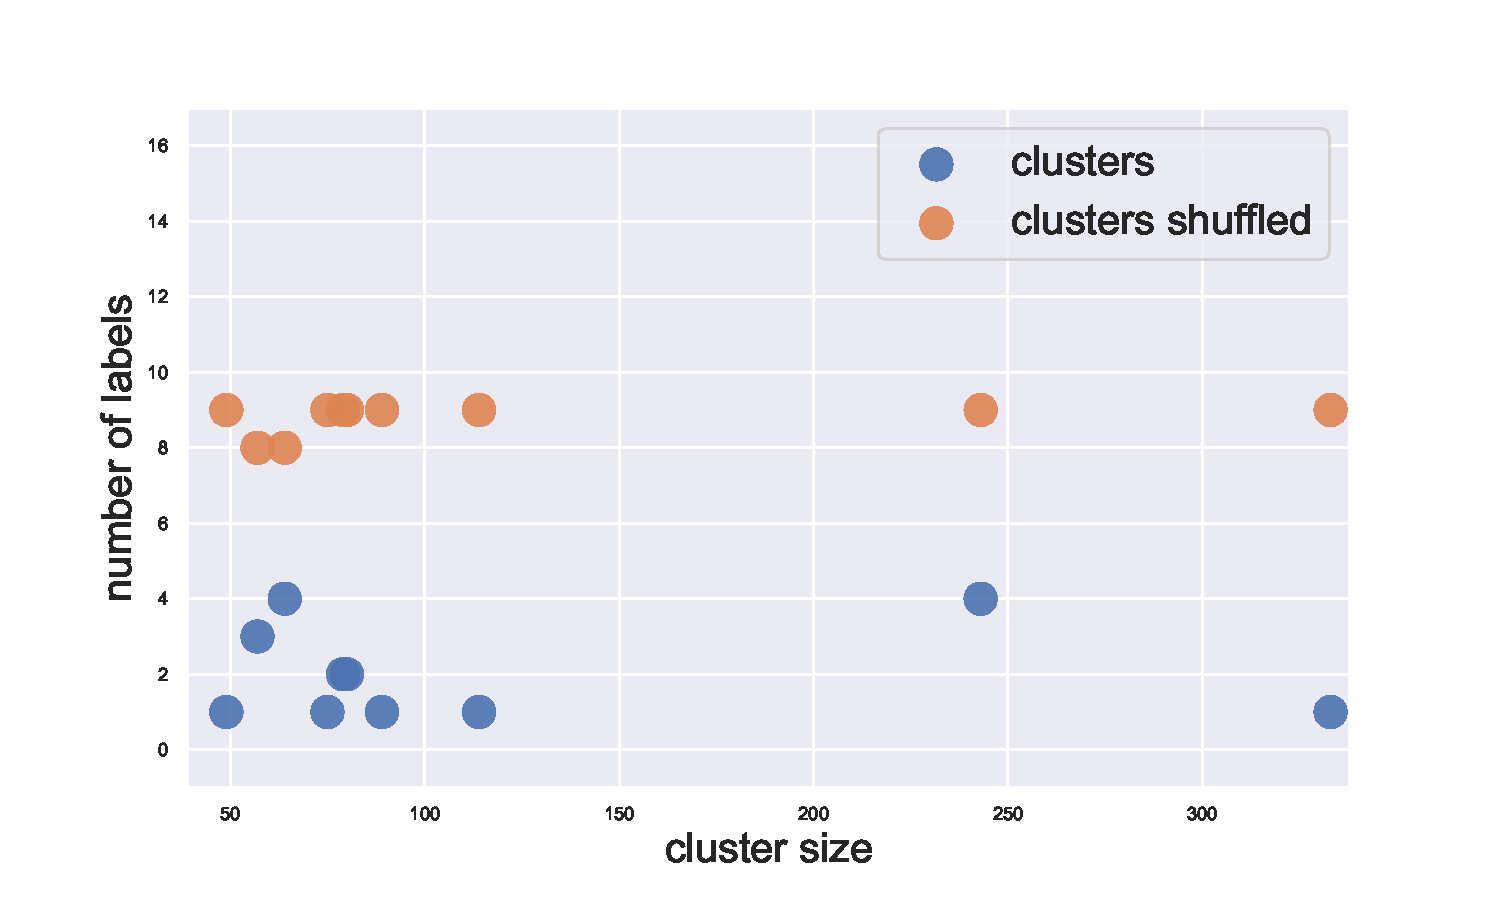
\includegraphics[width=0.9\linewidth]{pictures/topic/gtex/oversigma_10tissue/shuffledcluster_shuffle_label_size_l3_primary_site.pdf}
    \caption{Number of different labels in each cluster versus cluster size.}
    \label{fig:topic/gtex/oversigma_10tissue/shuffledcluster_shuffle_label_size_l3_primary_site}
\end{figure}
In figure~\ref{fig:topic/gtex/oversigma_10tissue/shuffledcluster_shuffle_label_size_l*} the same analysis for all the layer of the hierarchy. Even here the deeper level does not differ from the null model. Nevertheless in layers with higher V-measure score there is a strong signal that the reshuffling model is quite different from the real labels output.
\begin{figure}[htb!]
    \centering
    \begin{minipage}{0.45\textwidth}
    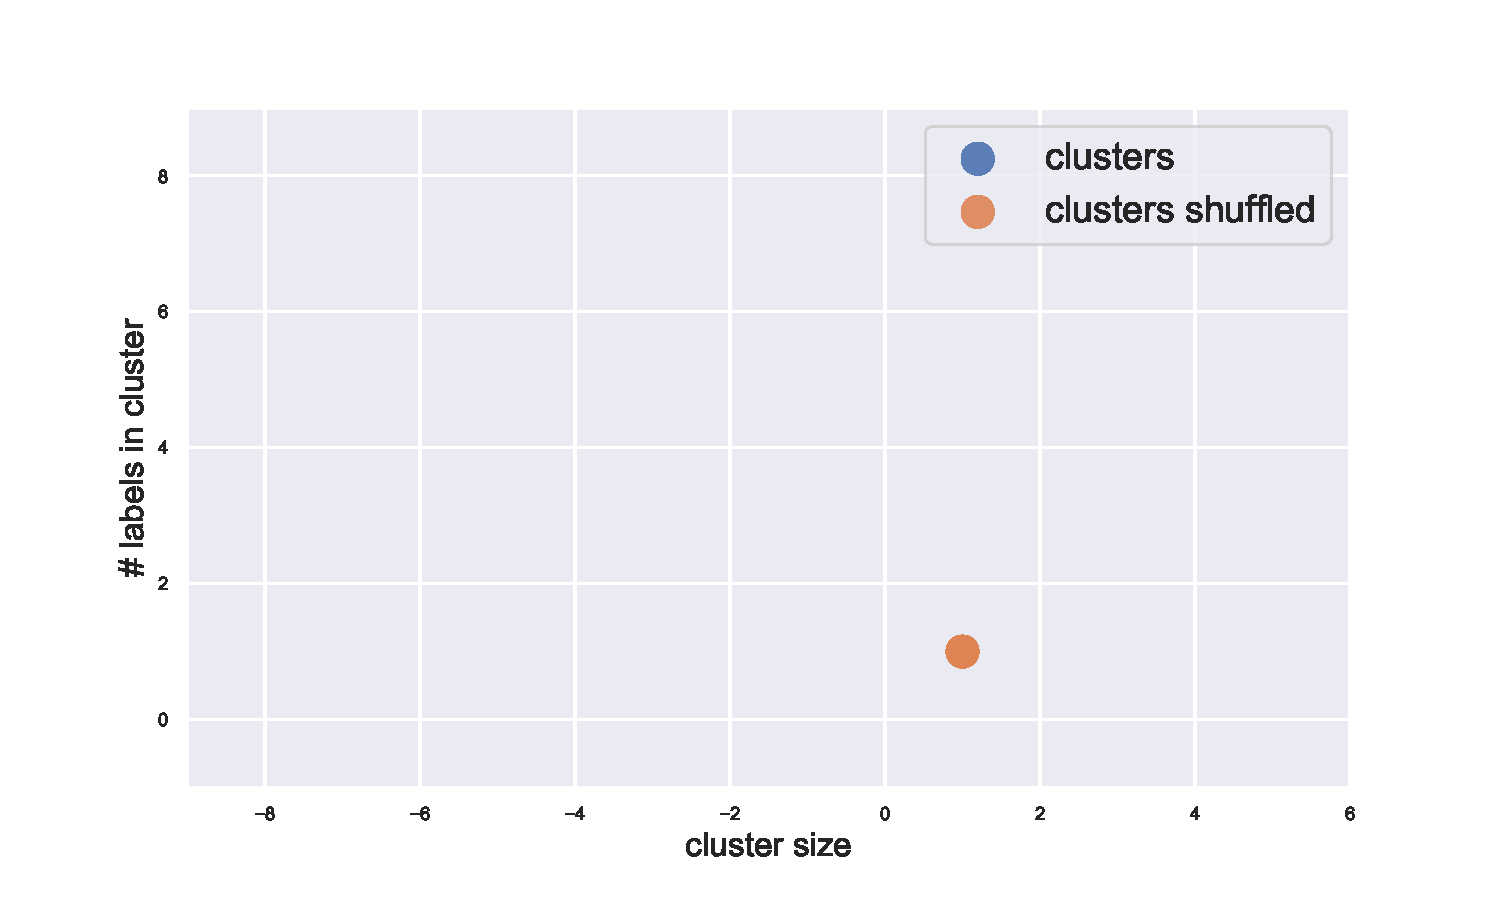
\includegraphics[width=0.9\linewidth]{pictures/topic/gtex/oversigma_10tissue/shuffledcluster_shuffle_label_size_l0_primary_site.pdf}
    \end{minipage}
    \hspace{3mm}
    \begin{minipage}{0.45\textwidth}
    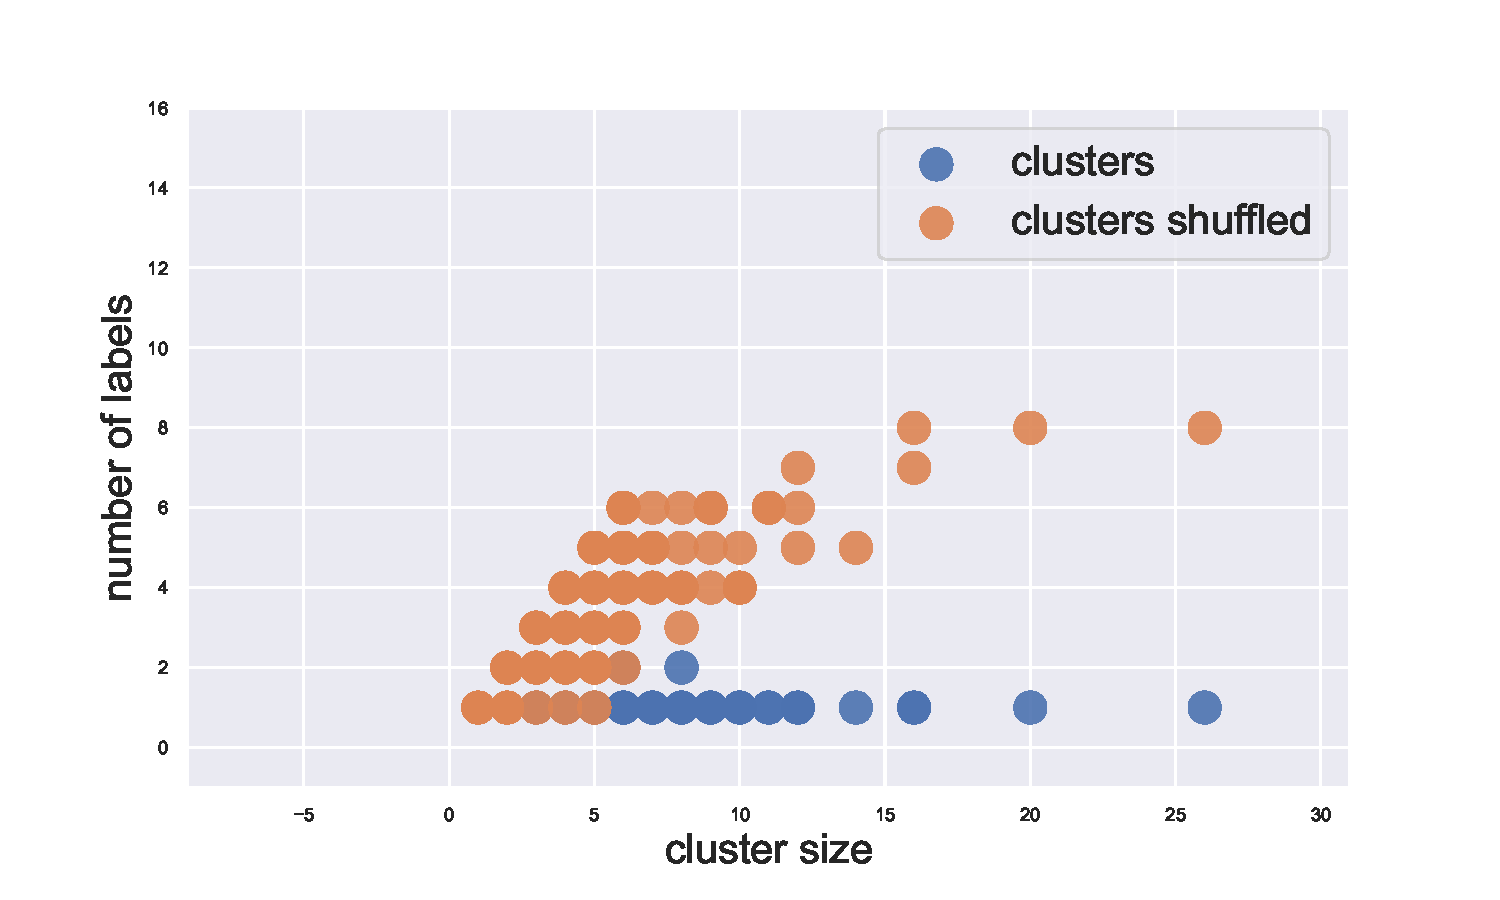
\includegraphics[width=0.9\linewidth]{pictures/topic/gtex/oversigma_10tissue/shuffledcluster_shuffle_label_size_l1_primary_site.pdf}
    \end{minipage}
    \\
    \begin{minipage}{0.45\textwidth}
    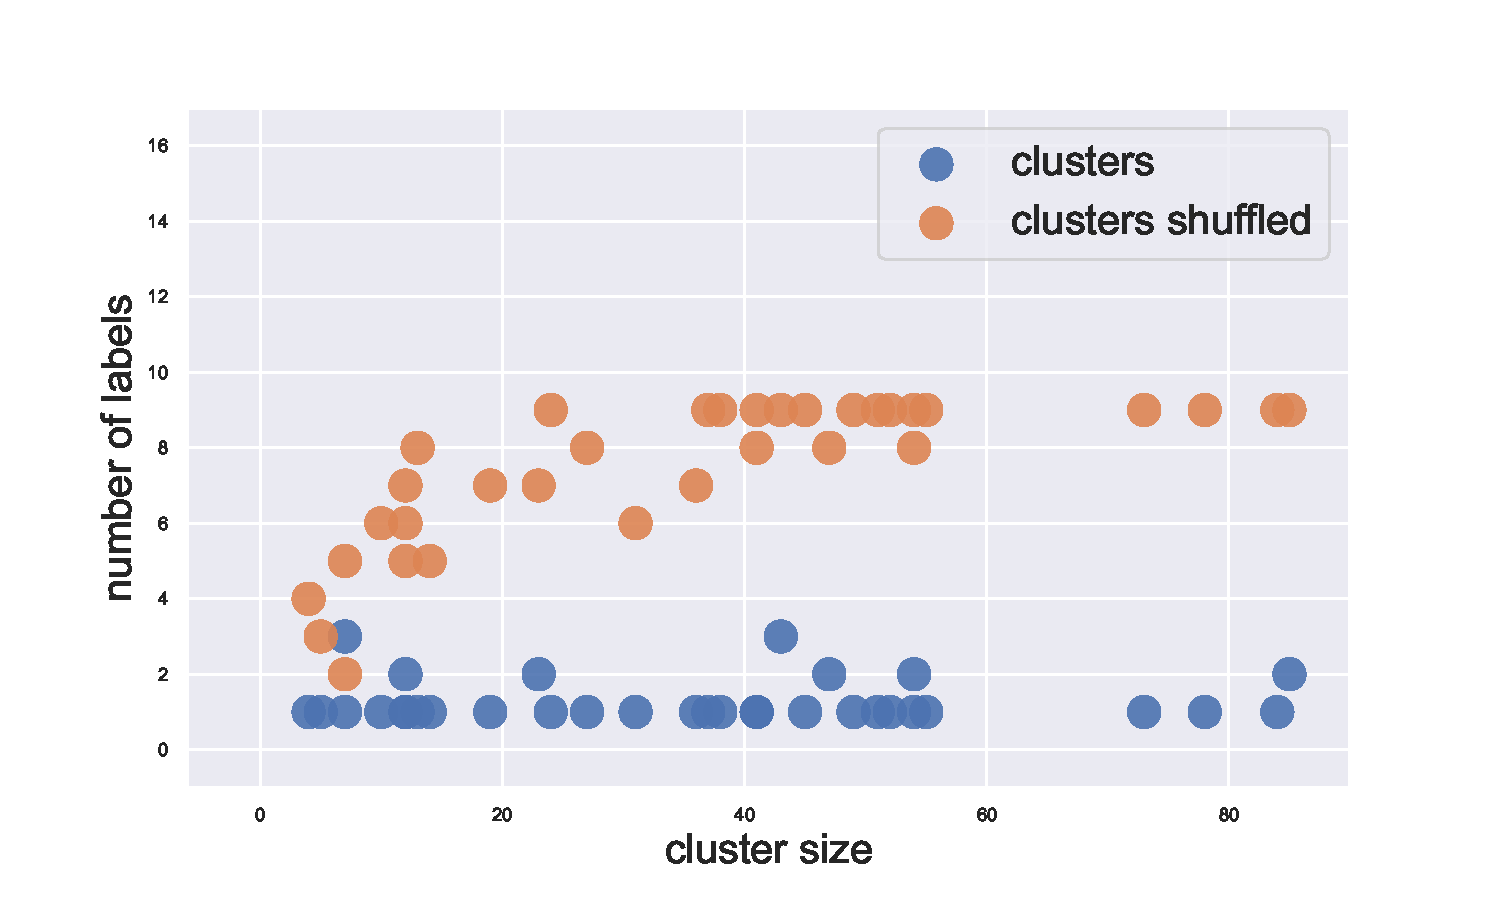
\includegraphics[width=0.9\linewidth]{pictures/topic/gtex/oversigma_10tissue/shuffledcluster_shuffle_label_size_l2_primary_site.pdf}
    \end{minipage}
    \hspace{3mm}
    \begin{minipage}{0.45\textwidth}
    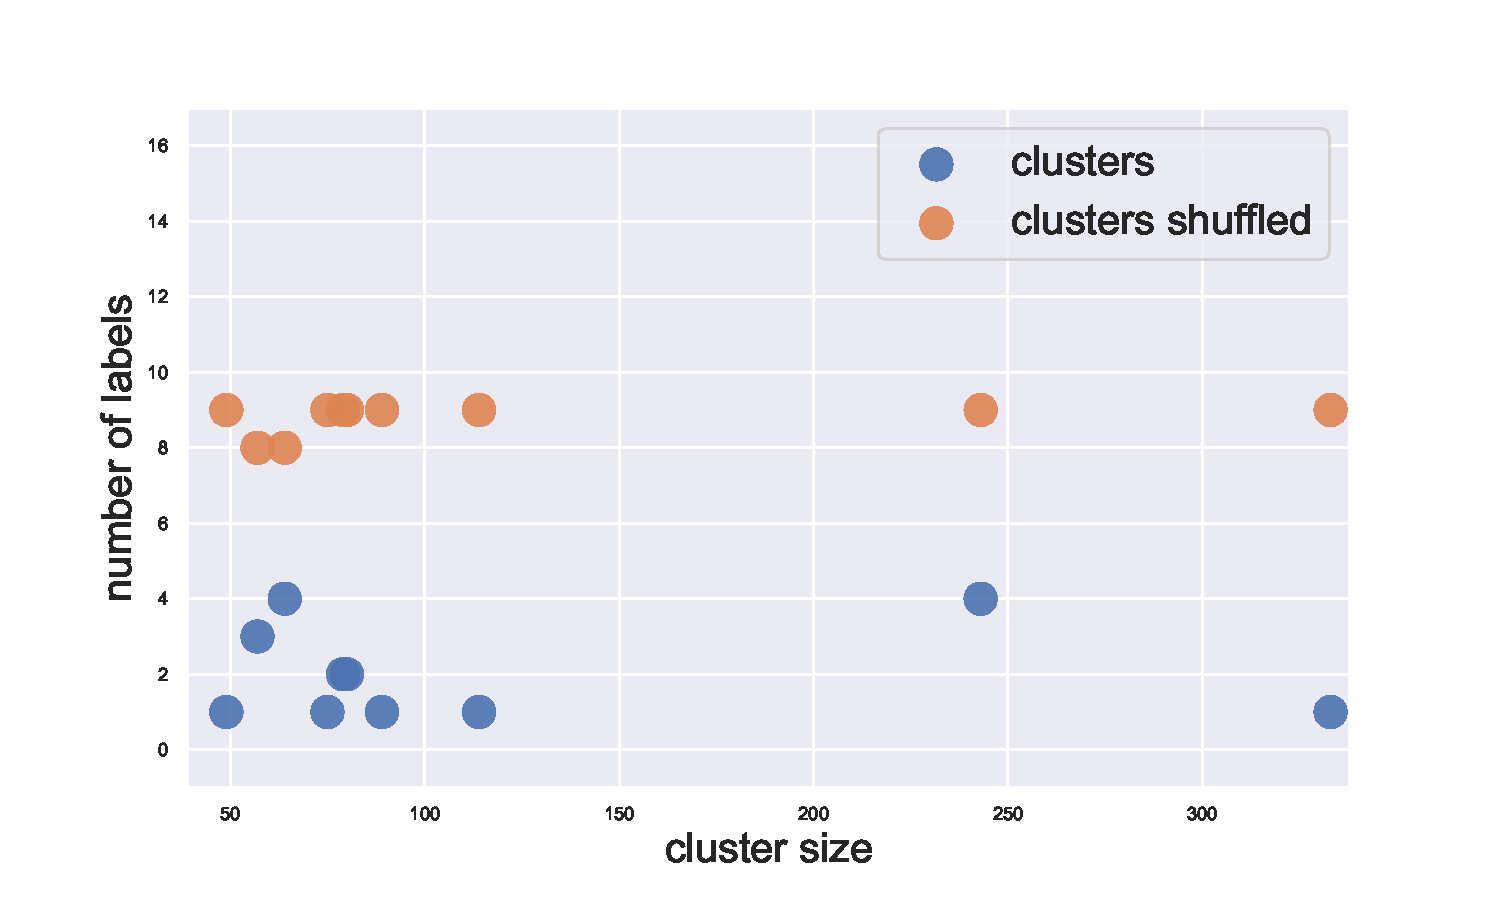
\includegraphics[width=0.9\linewidth]{pictures/topic/gtex/oversigma_10tissue/shuffledcluster_shuffle_label_size_l3_primary_site.pdf}
    \end{minipage}
\label{fig:topic/gtex/oversigma_10tissue/shuffledcluster_shuffle_label_size_l*}
\caption{Number of different labels in each cluster versus cluster size. From upper left the deeper layer than down right the upper one.}
\end{figure}

Having constructed the null model it is possible estimate the V-measure score also for the null model. The results are reported in figure~\ref{fig:topic/gtex/oversigma_10tissue/metric_scores_shuffle}. 
Moreover remembering the V-measure or normalized mutual information defined in~\ref{eq:mutualinformation} it is possible to estimate a mixed score which considers the homogeneity of primary site and the completeness of secondary site, doing so the score goes up if going deeper in the hierarchy the model makes more cluster with the same tissue but separates sub tissues. In fact it is not a big deal if one loses completeness regarding tissues (the model separates one big cluster full with the same label into two small ones) but gain information at the next magnification information. This is clear if one look at the big blood cluster that in the next level of the hierarchy is separated into two clusters of blood, one of whole blood and one of lymphocytes. The result is that this mixed score is the highest one.
\begin{figure}[htb!]
    \centering
    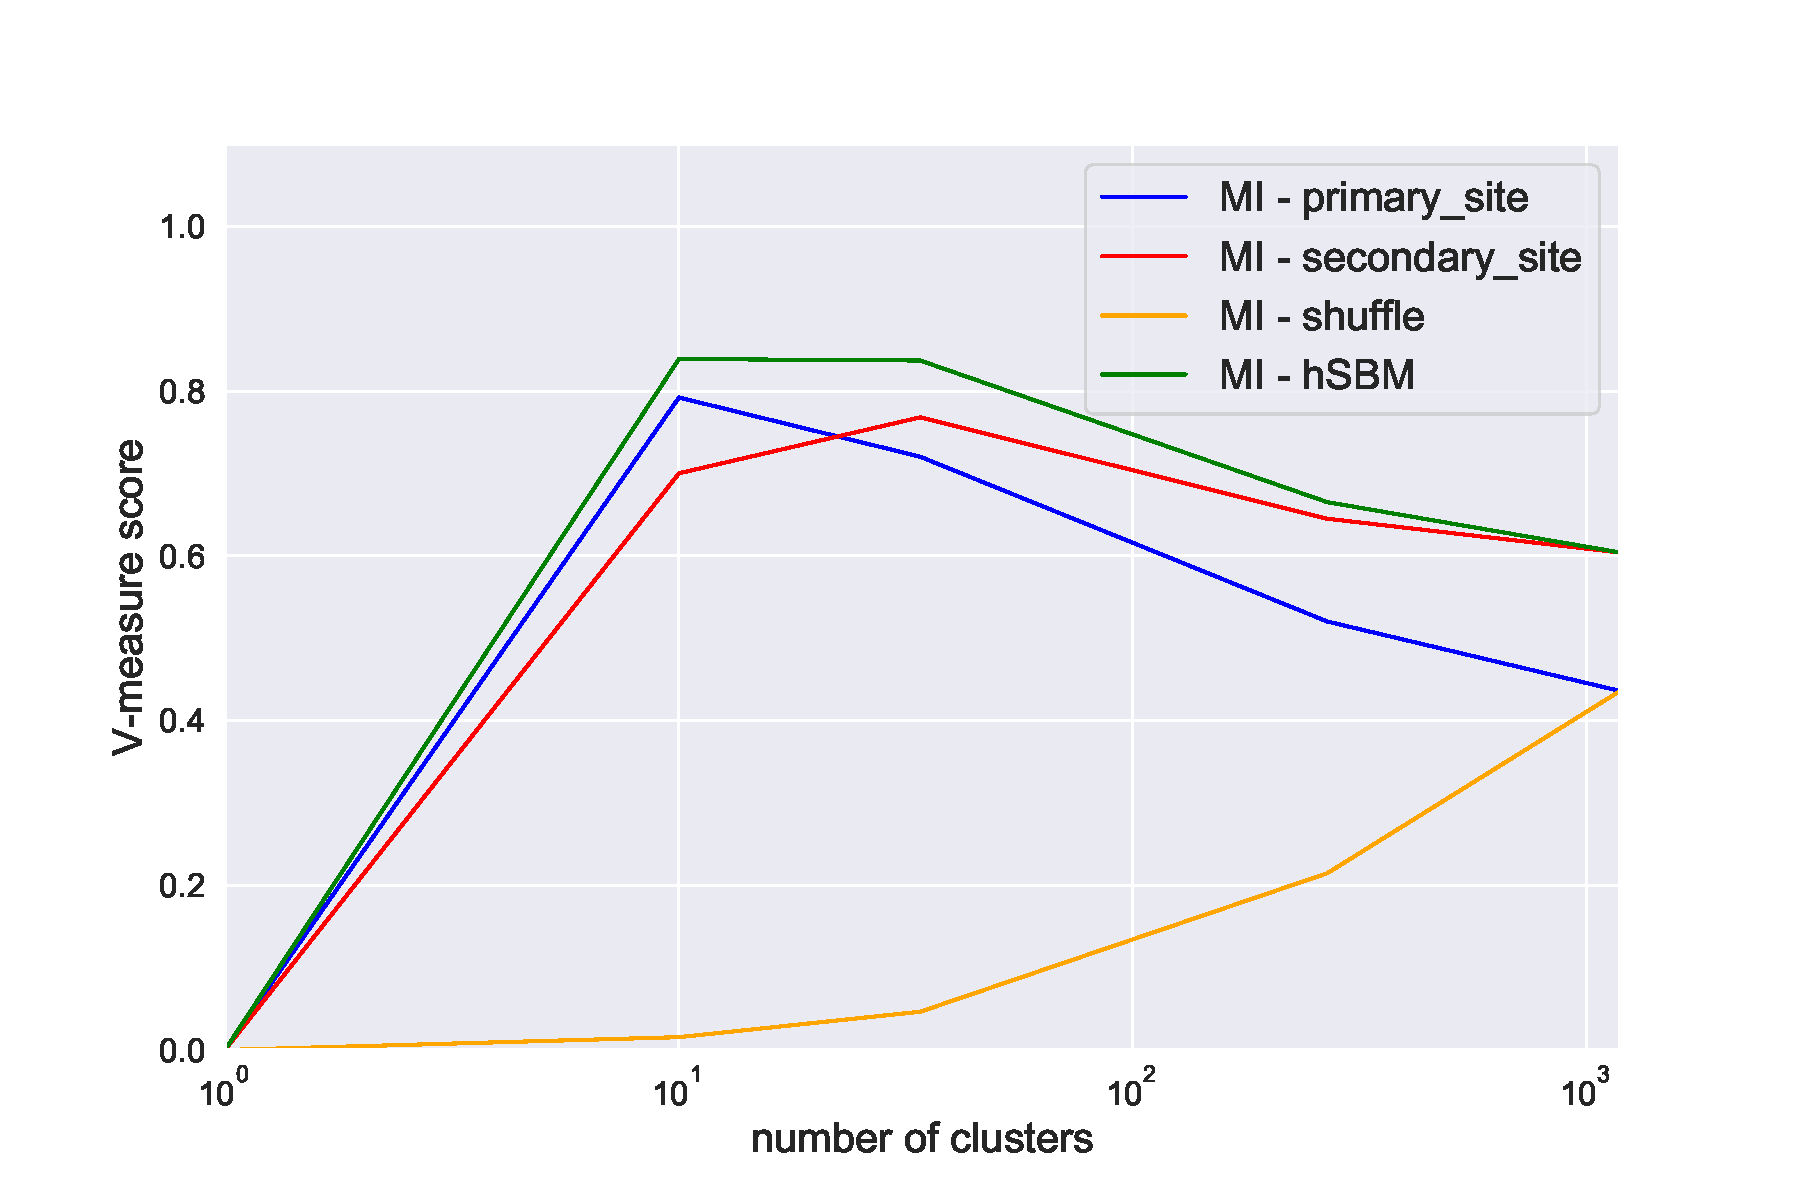
\includegraphics[width=0.9\linewidth]{pictures/topic/gtex/oversigma_10tissue/metric_scores_shuffle.pdf}
    \caption{Scores across hierarchy. The scored is compared with some random labels. In blue the score for the primary site labels, in red for the secondary site labels, in yellow the shuffled labels, in green the mixed score with primary homogeneity and secondary completeness.}
    \label{fig:topic/gtex/oversigma_10tissue/metric_scores_shuffle}
\end{figure}

\clearpage
\subsection{Standard algorithms}
At this point was verified that the model has got interesting output, it reaches high scores and has got a strong signal against null model, at least at some levels of the hierarchy. It is now interesting to compare it with standard and well-known similar algorithms.
First of all a comparison is made with hierarchical clustering. This is done using the standard scipy~\cite{jones2014scipy} package, the metrics used was the euclidean one and the linkage method was set to Ward. This is quite fast, it needs a couple of minutes on a dual core, 8GB memory machine.
In figure~\ref{fig:topic/gtex/oversigma_10tissue/metric_scores_hier} the comparison between this scores, the hierarchical algorithm performs worse than hierarchical stochastic block model and as highly expected better than the random model.
\begin{figure}[htb!]
    \centering
    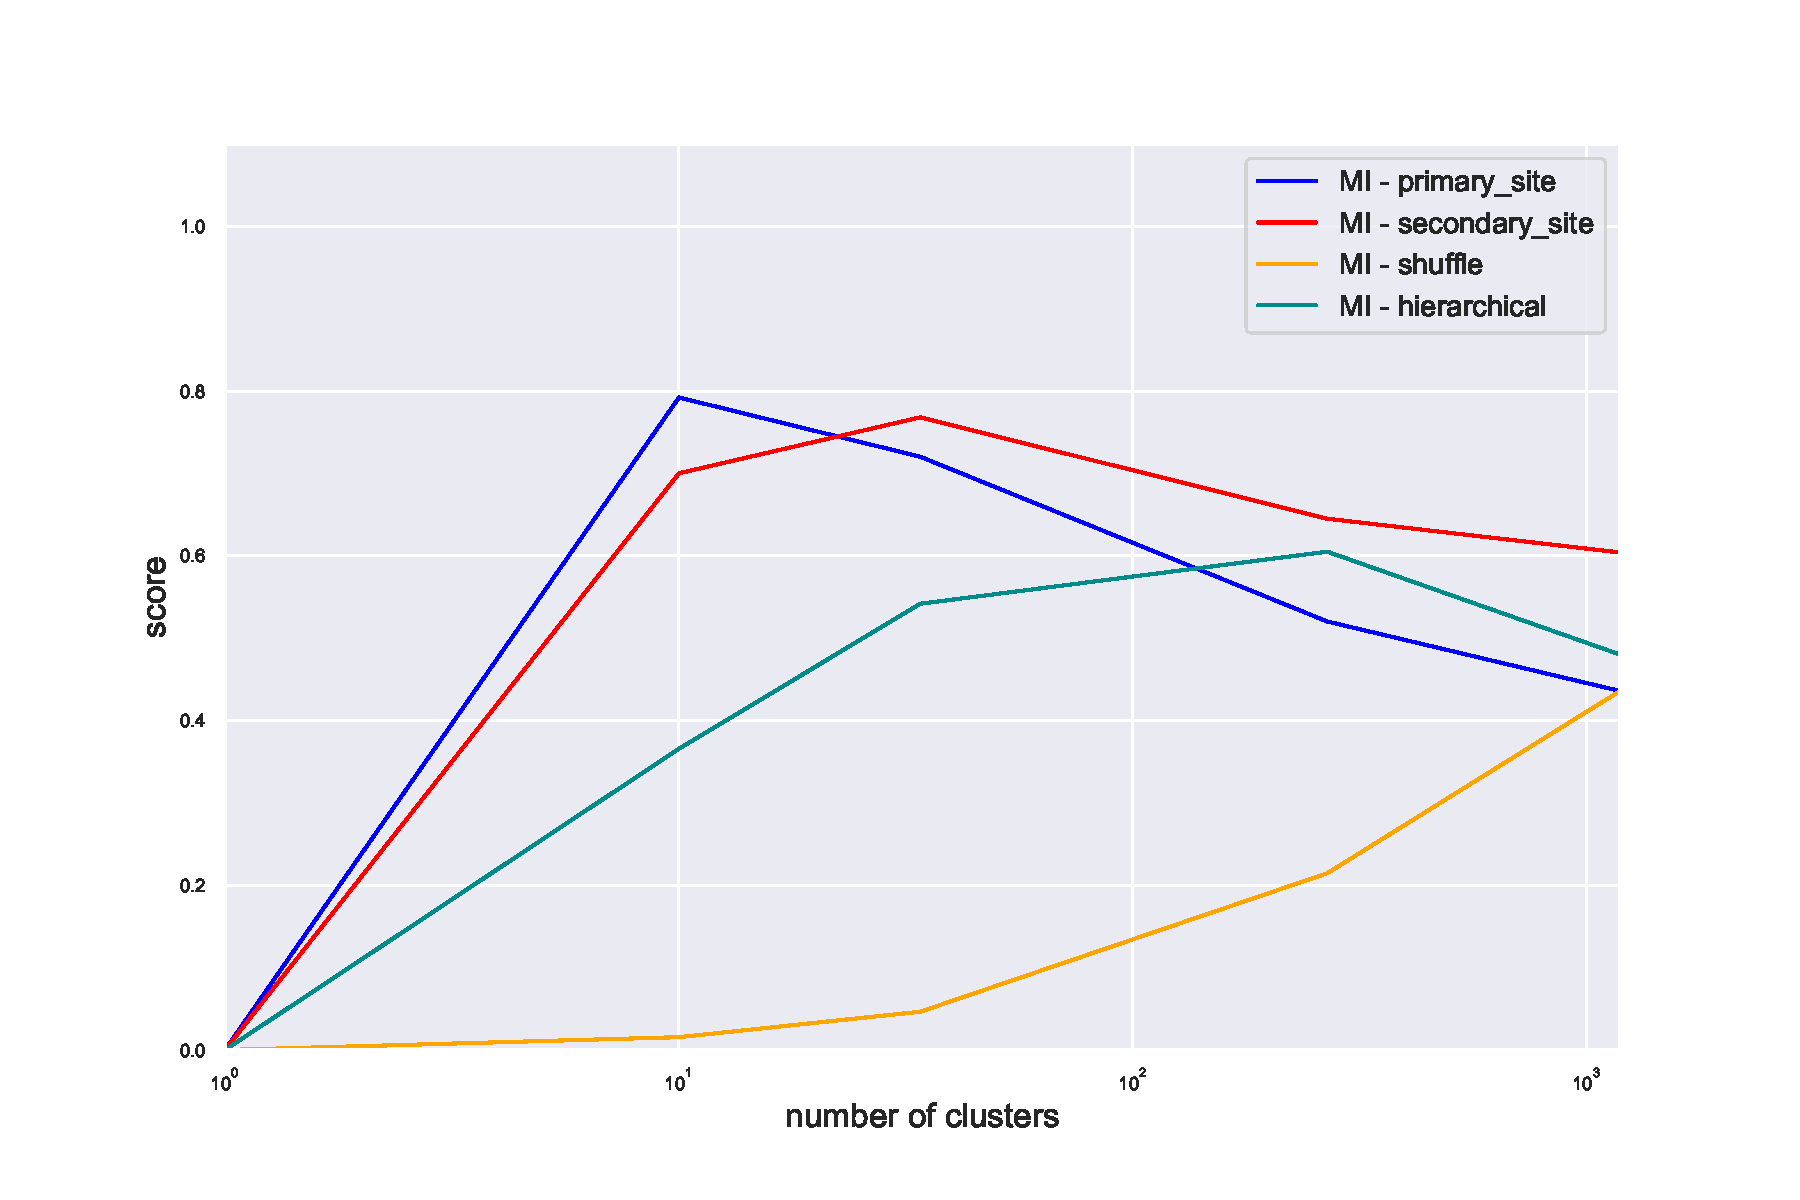
\includegraphics[width=0.9\linewidth]{pictures/topic/gtex/oversigma_10tissue/metric_scores_hier.pdf}
    \caption{Scores across hierarchy. The scored is compared with some random labels}
    \label{fig:topic/gtex/oversigma_10tissue/metric_scores_hier}
\end{figure}

Another very used and well-studied algorithm is Latent Dirichlet Allocation briefly described in~\ref{sec:lda}
\begin{figure}[htb!]
    \centering
    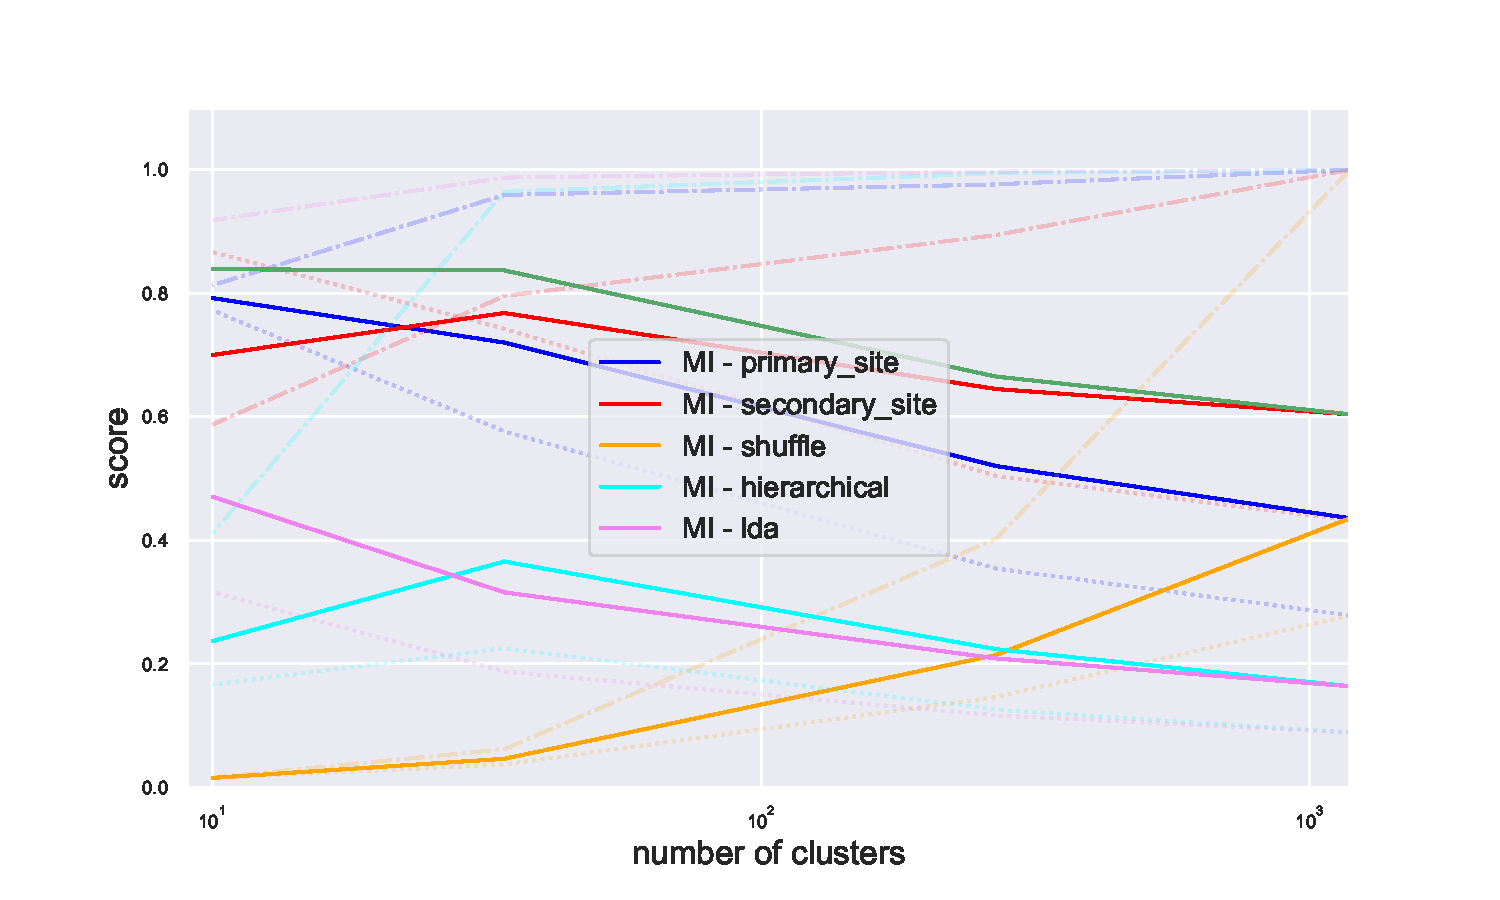
\includegraphics[width=0.9\linewidth]{pictures/topic/gtex/oversigma_10tissue/metric_scores_all.pdf}
    \caption{Scores across hierarchy. The scored is compared with some random labels}
    \label{fig:topic/gtex/oversigma_10tissue/metric_scores_all}
\end{figure}

\subsection{Topics}
\draft{Using gsea ~\cite{subramanian2005gene} as gene set ~\cite{Ardlie2015} enrichment test can be made from python \cite{Kuleshov2016}}

\begin{table}[htb!]
	\tiny
	\begin{center}
		\begin{tabular}{|c|c|c|}
			\hline
			Term & \multicolumn{1}{l|}{Adjusted P-value} & Gene\_set \\ \hline
			pancreas\_male\_60-69\_years & 1E-19 & GTEx\_Tissue\_Sample\_Gene\_Expression\_Profiles\_up \\ \hline
			pancreas\_female\_40-49\_years & 3E-19 & GTEx\_Tissue\_Sample\_Gene\_Expression\_Profiles\_up \\ \hline
			pancreas\_male\_40-49\_years & 5E-19 & GTEx\_Tissue\_Sample\_Gene\_Expression\_Profiles\_up \\ \hline
			pancreas\_male\_30-39\_years & 1E-18 & GTEx\_Tissue\_Sample\_Gene\_Expression\_Profiles\_up \\ \hline
			pancreas\_female\_20-29\_years & 1E-18 & GTEx\_Tissue\_Sample\_Gene\_Expression\_Profiles\_up \\ \hline
			pancreas\_male\_50-59\_years & 1E-18 & GTEx\_Tissue\_Sample\_Gene\_Expression\_Profiles\_up \\ \hline
			pancreas\_female\_30-39\_years & 1E-18 & GTEx\_Tissue\_Sample\_Gene\_Expression\_Profiles\_up \\ \hline
			pancreas\_male\_50-59\_years & 2E-18 & GTEx\_Tissue\_Sample\_Gene\_Expression\_Profiles\_up \\ \hline
			pancreas\_male\_40-49\_years & 2E-18 & GTEx\_Tissue\_Sample\_Gene\_Expression\_Profiles\_up \\ \hline
			pancreas\_male\_30-39\_years & 2E-18 & GTEx\_Tissue\_Sample\_Gene\_Expression\_Profiles\_up \\ \hline
			pancreas\_male\_50-59\_years & 2E-18 & GTEx\_Tissue\_Sample\_Gene\_Expression\_Profiles\_up \\ \hline
			pancreas\_female\_20-29\_years & 2E-18 & GTEx\_Tissue\_Sample\_Gene\_Expression\_Profiles\_up \\ \hline
			pancreas\_male\_40-49\_years & 3E-18 & GTEx\_Tissue\_Sample\_Gene\_Expression\_Profiles\_up \\ \hline
			pancreas\_female\_50-59\_years & 4E-18 & GTEx\_Tissue\_Sample\_Gene\_Expression\_Profiles\_up \\ \hline
			pancreas\_male\_50-59\_years & 4E-18 & GTEx\_Tissue\_Sample\_Gene\_Expression\_Profiles\_up \\ \hline
			pancreas\_male\_50-59\_years & 4E-18 & GTEx\_Tissue\_Sample\_Gene\_Expression\_Profiles\_up \\ \hline
			pancreas\_female\_60-69\_years & 5E-18 & GTEx\_Tissue\_Sample\_Gene\_Expression\_Profiles\_up \\ \hline
			pancreas\_female\_50-59\_years & 5E-18 & GTEx\_Tissue\_Sample\_Gene\_Expression\_Profiles\_up \\ \hline
			pancreas\_male\_50-59\_years & 5E-18 & GTEx\_Tissue\_Sample\_Gene\_Expression\_Profiles\_up \\ \hline
			pancreas\_male\_30-39\_years & 6E-18 & GTEx\_Tissue\_Sample\_Gene\_Expression\_Profiles\_up \\ \hline
		\end{tabular}
	\end{center}
	\caption{Enrichment}
	\label{topic/enrich/pancreas}
\end{table}

\begin{table}[htb!]
	\tiny
	\begin{center}
		\begin{tabular}{|c|c|c|}
			\hline
			Term & \multicolumn{1}{l|}{Adjusted P-value} & Gene\_set \\ \hline
			brain\_female\_40-49\_years & 6E-05 & GTEx\_Tissue\_Sample\_Gene\_Expression\_Profiles\_up \\ \hline
			brain\_male\_50-59\_years & 6E-05 & GTEx\_Tissue\_Sample\_Gene\_Expression\_Profiles\_up \\ \hline
			brain\_female\_60-69\_years & 6E-05 & GTEx\_Tissue\_Sample\_Gene\_Expression\_Profiles\_up \\ \hline
			brain\_female\_60-69\_years & 6E-05 & GTEx\_Tissue\_Sample\_Gene\_Expression\_Profiles\_up \\ \hline
			brain\_female\_60-69\_years & 6E-05 & GTEx\_Tissue\_Sample\_Gene\_Expression\_Profiles\_up \\ \hline
			brain\_female\_40-49\_years & 6E-05 & GTEx\_Tissue\_Sample\_Gene\_Expression\_Profiles\_up \\ \hline
			brain\_female\_40-49\_years & 6E-05 & GTEx\_Tissue\_Sample\_Gene\_Expression\_Profiles\_up \\ \hline
			brain\_female\_60-69\_years & 6E-05 & GTEx\_Tissue\_Sample\_Gene\_Expression\_Profiles\_up \\ \hline
			brain\_male\_60-69\_years & 6E-05 & GTEx\_Tissue\_Sample\_Gene\_Expression\_Profiles\_up \\ \hline
			brain\_male\_50-59\_years & 6E-05 & GTEx\_Tissue\_Sample\_Gene\_Expression\_Profiles\_up \\ \hline
			brain\_male\_50-59\_years & 6E-05 & GTEx\_Tissue\_Sample\_Gene\_Expression\_Profiles\_up \\ \hline
			brain\_male\_60-69\_years & 7E-05 & GTEx\_Tissue\_Sample\_Gene\_Expression\_Profiles\_up \\ \hline
			brain\_male\_50-59\_years & 7E-05 & GTEx\_Tissue\_Sample\_Gene\_Expression\_Profiles\_up \\ \hline
			brain\_male\_20-29\_years & 7E-05 & GTEx\_Tissue\_Sample\_Gene\_Expression\_Profiles\_up \\ \hline
			brain\_female\_60-69\_years & 8E-05 & GTEx\_Tissue\_Sample\_Gene\_Expression\_Profiles\_up \\ \hline
			brain\_female\_60-69\_years & 8E-05 & GTEx\_Tissue\_Sample\_Gene\_Expression\_Profiles\_up \\ \hline
			brain\_female\_60-69\_years & 1E-04 & GTEx\_Tissue\_Sample\_Gene\_Expression\_Profiles\_up \\ \hline
			brain\_female\_60-69\_years & 1E-04 & GTEx\_Tissue\_Sample\_Gene\_Expression\_Profiles\_up \\ \hline
			brain\_female\_60-69\_years & 1E-04 & GTEx\_Tissue\_Sample\_Gene\_Expression\_Profiles\_up \\ \hline
			brain\_male\_60-69\_years & 1E-04 & GTEx\_Tissue\_Sample\_Gene\_Expression\_Profiles\_up \\ \hline
		\end{tabular}
	\end{center}
	\caption{Enrichment}
	\label{topic/enrich/brain}
\end{table}

\begin{table}[htb!]
	\centering
	\tiny
	\begin{tabular}{|c|c|c|}
		\hline
		Term & \multicolumn{1}{l|}{Adjusted P-value} & Gene\_set \\ \hline
		blood\_male\_50-59\_years & 3E-23 & GTEx\_Tissue\_Sample\_Gene\_Expression\_Profiles\_up \\ \hline
		blood\_male\_50-59\_years & 3E-23 & GTEx\_Tissue\_Sample\_Gene\_Expression\_Profiles\_up \\ \hline
		blood\_male\_40-49\_years & 3E-21 & GTEx\_Tissue\_Sample\_Gene\_Expression\_Profiles\_up \\ \hline
		blood\_male\_60-69\_years & 9E-21 & GTEx\_Tissue\_Sample\_Gene\_Expression\_Profiles\_up \\ \hline
		blood\_male\_40-49\_years & 3E-20 & GTEx\_Tissue\_Sample\_Gene\_Expression\_Profiles\_up \\ \hline
		blood\_female\_60-69\_years & 4E-20 & GTEx\_Tissue\_Sample\_Gene\_Expression\_Profiles\_up \\ \hline
		blood\_male\_60-69\_years & 4E-20 & GTEx\_Tissue\_Sample\_Gene\_Expression\_Profiles\_up \\ \hline
		blood\_female\_50-59\_years & 5E-20 & GTEx\_Tissue\_Sample\_Gene\_Expression\_Profiles\_up \\ \hline
		blood\_female\_50-59\_years & 1E-19 & GTEx\_Tissue\_Sample\_Gene\_Expression\_Profiles\_up \\ \hline
		blood\_male\_60-69\_years & 1E-19 & GTEx\_Tissue\_Sample\_Gene\_Expression\_Profiles\_up \\ \hline
		blood\_male\_60-69\_years & 1E-19 & GTEx\_Tissue\_Sample\_Gene\_Expression\_Profiles\_up \\ \hline
		blood\_female\_60-69\_years & 1E-19 & GTEx\_Tissue\_Sample\_Gene\_Expression\_Profiles\_up \\ \hline
		blood\_male\_60-69\_years & 2E-19 & GTEx\_Tissue\_Sample\_Gene\_Expression\_Profiles\_up \\ \hline
		blood\_male\_50-59\_years & 2E-19 & GTEx\_Tissue\_Sample\_Gene\_Expression\_Profiles\_up \\ \hline
		blood\_female\_40-49\_years & 2E-19 & GTEx\_Tissue\_Sample\_Gene\_Expression\_Profiles\_up \\ \hline
		blood\_female\_40-49\_years & 2E-19 & GTEx\_Tissue\_Sample\_Gene\_Expression\_Profiles\_up \\ \hline
		blood\_female\_60-69\_years & 2E-19 & GTEx\_Tissue\_Sample\_Gene\_Expression\_Profiles\_up \\ \hline
		blood\_male\_30-39\_years & 3E-19 & GTEx\_Tissue\_Sample\_Gene\_Expression\_Profiles\_up \\ \hline
		blood\_female\_50-59\_years & 5E-19 & GTEx\_Tissue\_Sample\_Gene\_Expression\_Profiles\_up \\ \hline
		blood\_female\_60-69\_years & 5E-19 & GTEx\_Tissue\_Sample\_Gene\_Expression\_Profiles\_up \\ \hline
	\end{tabular}
	\label{topic/enrich/blood}
	\caption{Enrichment}
\end{table}

Enrichment test are made once for each topic, starting from the layer with more genes per 
single topic. Test are made across multiple categories.
